\documentclass{scrreprt}
\usepackage{scrhack}
\usepackage{listings}
\usepackage{underscore}
\usepackage[margin=2cm]{geometry}
\usepackage{graphicx}
\usepackage[bookmarks=true]{hyperref}
\usepackage[utf8]{inputenc}
\usepackage[english]{babel}
\usepackage[super]{nth}
\usepackage{placeins}
\usepackage[table,xcdraw]{xcolor}
\usepackage{array}
\usepackage{float}
\usepackage{xcolor,listings}
\usepackage{textcomp}
\usepackage{color}
\usepackage{pdfpages}
% \usepackage[formats]{listings}

\usepackage{etoolbox}
\makeatletter
\patchcmd{\scr@startchapter}{\if@openright\cleardoublepage\else\clearpage\fi}{}{}{}
\makeatother


\setlength{\parindent}{0em}
\setlength{\parskip}{1.0em}

\definecolor{mygreen}{rgb}{0,0.6,0}
\definecolor{mygray}{rgb}{0.5,0.5,0.5}
\definecolor{mymauve}{rgb}{0.58,0,0.82}
\definecolor{darkgray}{rgb}{.4,.4,.4}
\definecolor{purple}{rgb}{0.65, 0.12, 0.82}

\lstdefinelanguage{JavaScript}{
keywords={typeof, new, true, false, catch, function, return, null, catch, switch, var, if, in, while, do, else, case, break},
keywordstyle=\color{blue}\bfseries,
ndkeywords={class, export, boolean, throw, implements, import, this},
ndkeywordstyle=\color{darkgray}\bfseries,
identifierstyle=\color{black},
sensitive=false,
comment=[l]{//},
morecomment=[s]{/*}{*/},
commentstyle=\color{purple}\ttfamily,
stringstyle=\color{red}\ttfamily,
morestring=[b]',
morestring=[b]"
}

\lstset{
language=JavaScript,
extendedchars=true,
basicstyle=\footnotesize\ttfamily,
showstringspaces=false,
showspaces=false,
numbers=left,
numberstyle=\footnotesize,
numbersep=9pt,
tabsize=2,
breaklines=true,
showtabs=false,
frame=single, 
captionpos=b,
breaklines=true,
postbreak=\mbox{\textcolor{red}{$\hookrightarrow$}\space},
}

\addtokomafont{disposition}{\rmfamily}
%}
\usepackage{hyperref}

\pagenumbering{gobble}


\title{F21DV Coursework Lab 4 Report}
\author{Jonathan Song Yang, Lee (H00255553)}
\date{Demonstrated to: Dr. Benjamin Kenwright (08/04/2022)}

\begin{document}


\includepdf[pages={1}]{images/SD.pdf}

\maketitle

\newpage
\tableofcontents

\pagenumbering{arabic}


\newpage
\chapter{Introduction}
Lab 4 focuses on using the general visualization skill set obtained from the past 3 Labs, to design a complex, dynamic and interactive visualization webpage. 
\par GitHub Repo: \href{https://github.com/jonleesy/F21DV-Coursework}{https://github.com/jonleesy/F21DV-Coursework}
\par GitHub Pages: \href{https://jonleesy.github.io/F21DV-Coursework/public}{https://jonleesy.github.io/F21DV-Coursework/public}

\section{Set Up}
\subsection{Layout Set Up}
The application uses \verb|CSS| grid to drive its layout, and through the use of \verb|CSS| and \verb|JavaScript| DOM, a generalized function was used to create divs as shown in line 8 - 13 in listing \ref{lst:graph-scale}, where in line 20 onwards shows its implementation. 
\lstinputlisting[firstline = 9, lastline = 31, label = {lst:graph-scale}, caption = {Abstract of Systematic Div Creation}]{../../public/js/part4/functions.js}

\subsection{Modules Set Up}
The application is set up to be event-driven, where independent modules were used to process different segments within the application, and functions could be reused through different call-back contexts. Within each module, there exist an entry point \verb|setup()| function, and for some an additional \verb|update()| function. 
\lstinputlisting[firstline = 6, lastline = 27, label = {lst:setup}, caption = {Abstract of Entry Point Code}]{../../public/js/part4/main.js}
From listing \ref{lst:setup}, it could be seen that the entry point for all modules is through a \verb|setup()| function. 

\subsection{Testing Set Up}
Testings were mainly user driven. However, to ensure that code quality is up to standard, a local instance of \verb|ESLint|, \verb|Prettier| and \verb|SonarQube| was used to scan for vulnerability in code and ensure that best programming practices were used. The user testing and development was also done on a Mozilla based web browser.
\begin{figure}[H]
    \centering
    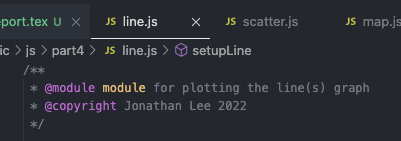
\includegraphics[width = 0.8\textwidth]{images/testing.png}
    \label{fig:Testing}
    \caption{JSDoc Module and Copyright}
\end{figure}

As shown in figure \ref{fig:Testing}, I have also added on \verb|JSDoc| style \verb|@module| and \verb|@copyright| descriptions to the top of each module file specifying its purposes, after the discussion during the demo. 

\subsection{Data Set Up}
\verb|Python| was used to pre-process the World Development Indicator dataset to shorten loading times. The data set would not be provided due to its sheer size, but the example of python code used to filter the data set is as below in listing \ref{lst:python}, only filtering for what is needed within the application.
\begin{lstlisting}[label = {lst:python}, caption = {Python Pre-Processing}]
import pandas as pd

# read csv using pd
# Data will have to be download from https://databank.worldbank.org/source/world-development-indicators# and redirected. 
df = pd.read_csv('wdi_raw.csv')

# filter df
list_of_series_code = ['NY.GDP.PCAP.KD', 'EN.POP.DNST']
new_df = df[df['Indicator Code'].isin(list_of_series_code)]

# write to csv
new_df.to_csv('wdi.csv', index=False)
\end{lstlisting}

\chapter{The Application and Its Feature}
\begin{figure}[H]
    \centering
    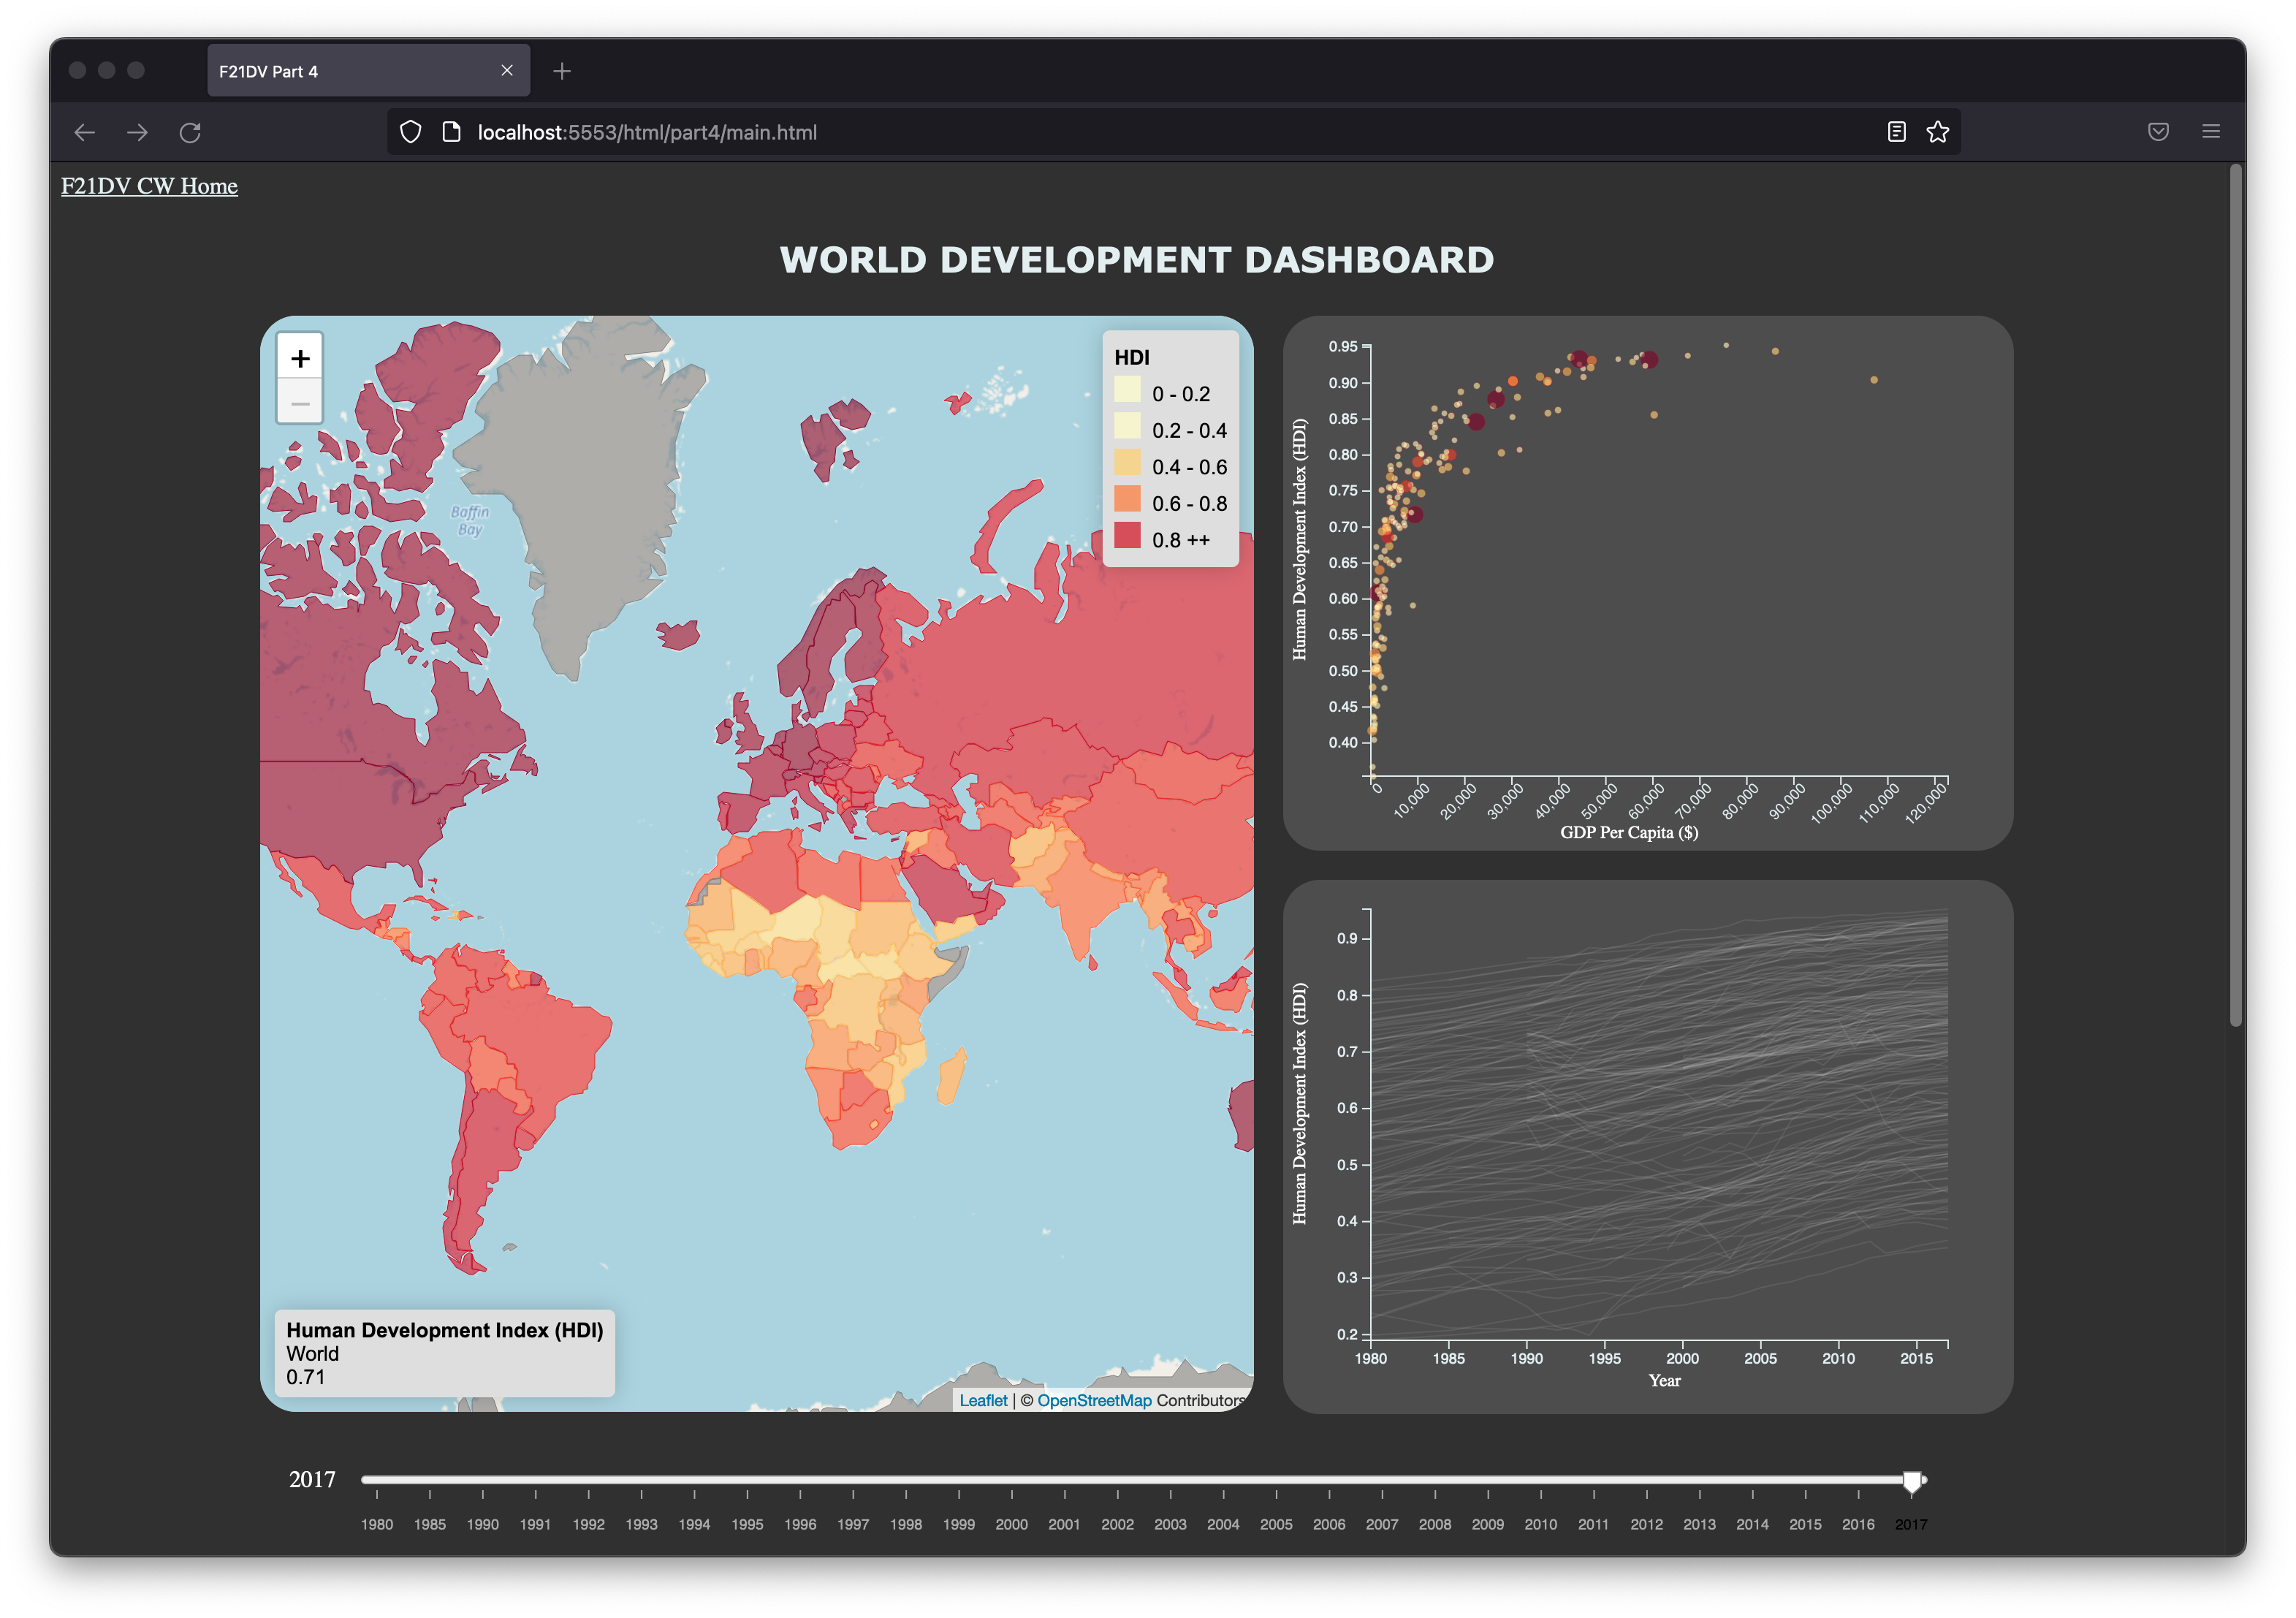
\includegraphics[width = 0.8\textwidth]{images/main.png}
    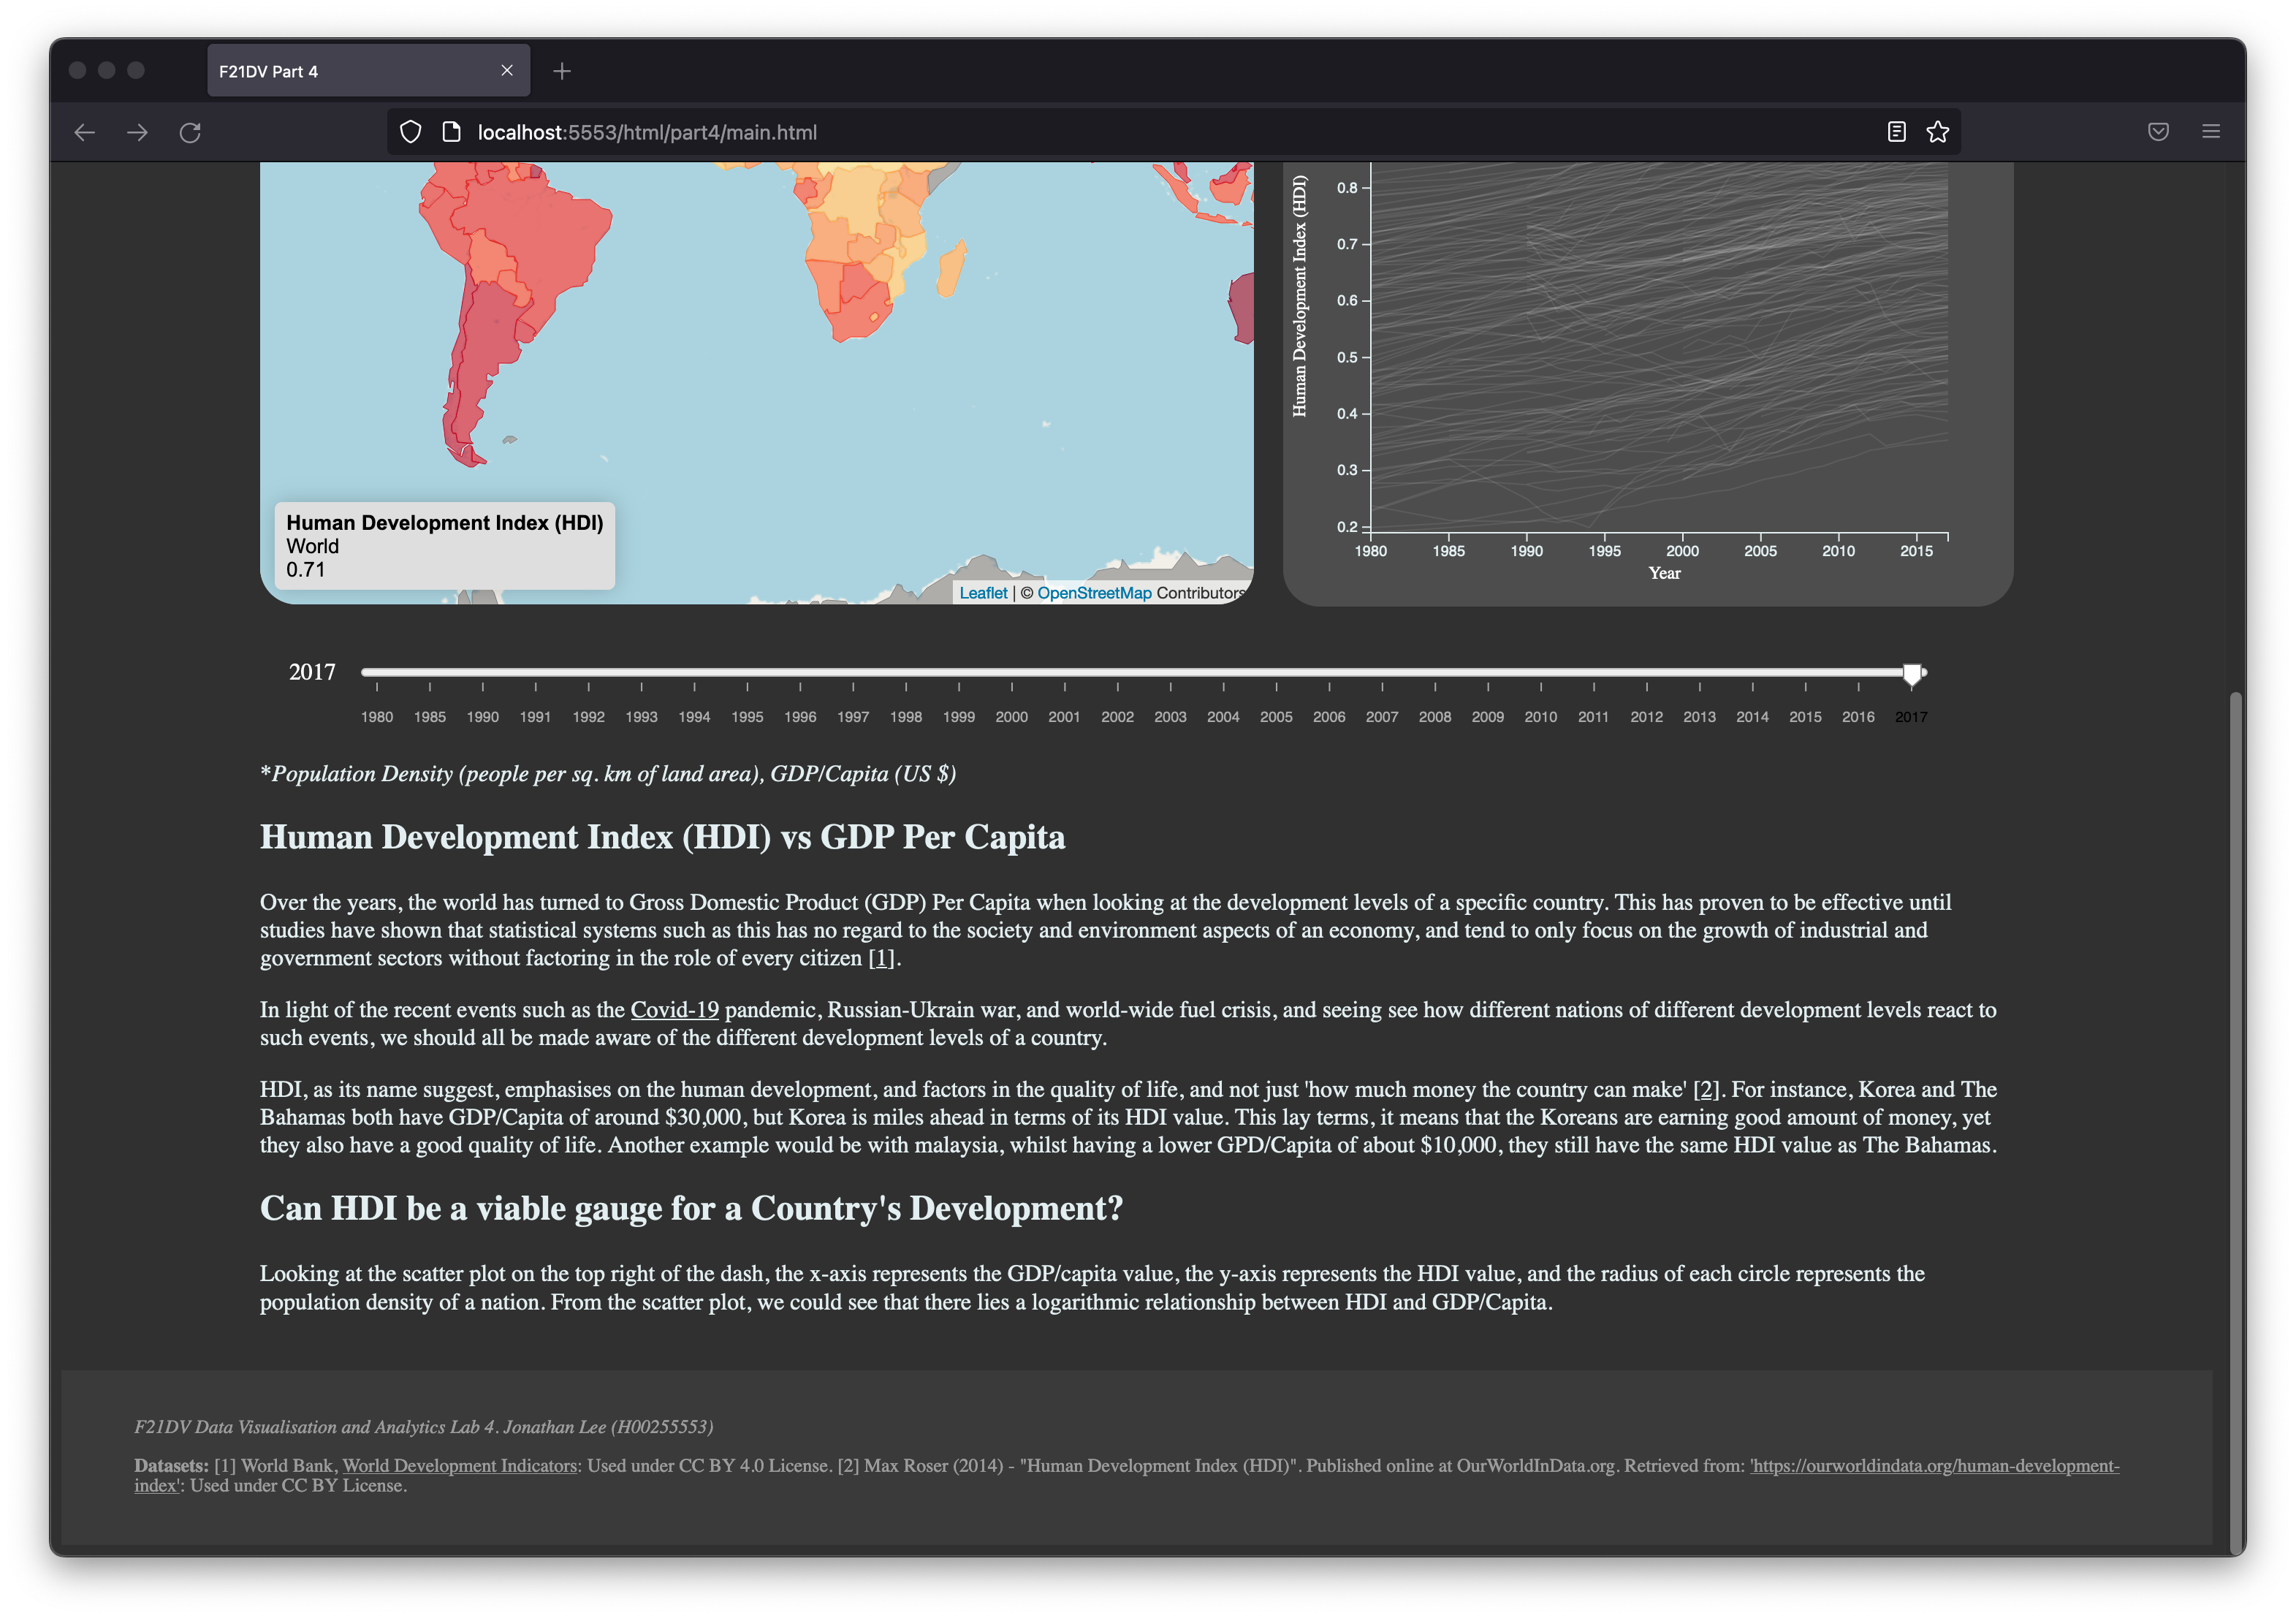
\includegraphics[width = 0.8\textwidth]{images/main_2.png}
    \label{fig:main}
    \caption{Main Dashboard Layout}
\end{figure}
Figure \ref{fig:main} shows the main layout of the application dashboard, mainly consisting of the map, scatter plot, multi-line chart, timeline slider, and a write-up of the dashboard. 

The main idea behind choosing to look into the two main development indicator, HDI and GDP/Capita, was inspired by the recent world events happening around us, and hoping that this would heighten our concerns to the different development levels of different countries. For instance, a country with low development index generally responded poorly to the Covid-19 pandemic. With lack of reach for vaccinations in the early days, and high population densities, these countries were hit with high virus reproduction rates and relatively worse symptoms as a result of infection. On the other hand a well-developed country with low population density and reach for advanced medical technologies were able to roll out vaccination campaigns quickly, and prevent a far worse transmission of the virus. 

These are all factors that should be put towards the calculation of a country's development index, and not just in layman terms `how much money does the country make in a year'. Hence, this dashboard focuses on the comparison of the use widely used Gross Domestic Product (GDP) per Capita (US \$) and Human Development Index (HDI) as a more viable indicator for development. 

\section{Map}
\begin{figure}[H]
    \centering
    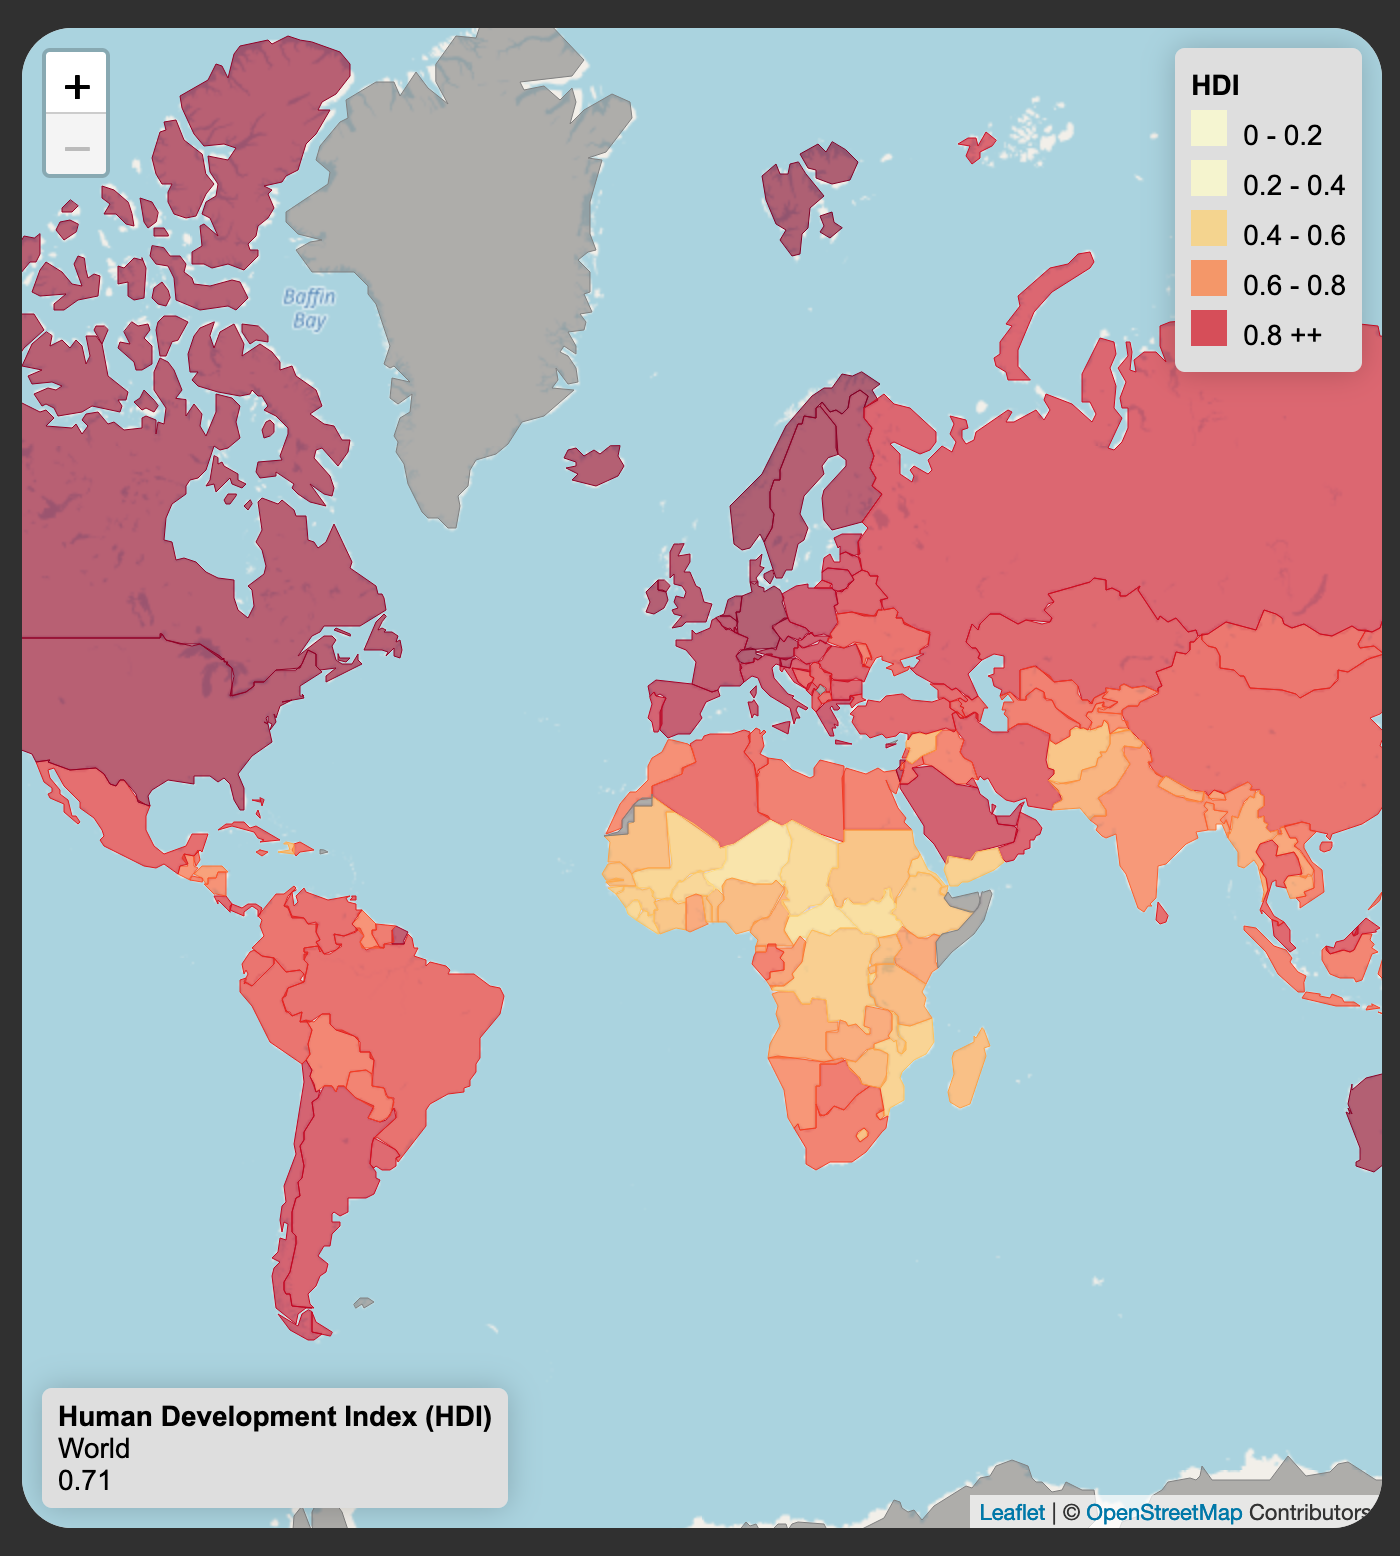
\includegraphics[width = 0.4\textwidth]{images/map_1.png}
    \label{fig:map}
    \caption{Map Container}
\end{figure}
The map shown in figure \ref{fig:map} was implemented using the \verb|leaflet| and \verb|d3.js| library, as shown in listing \ref*{lst:setup-map}.
\lstinputlisting[firstline = 186, lastline = 200, label = {lst:setup-map}, caption = {Abstract of map setup}]{../../public/js/part4/map.js}
Upon the setup of the map, using the \verb|L.control()| and \verb|L.onAdd()| functions, we have created both the Tooltip on the bottom left, and legend on the top right. Each layer of the map were also assigned unique class values such as \verb|`map-path-${countryCode}'|, and this is for the ease of performing style updates on individual layers. 

\subsection{Map, Scatter, Line Mouse Event}
\begin{figure}[H]
    \centering
    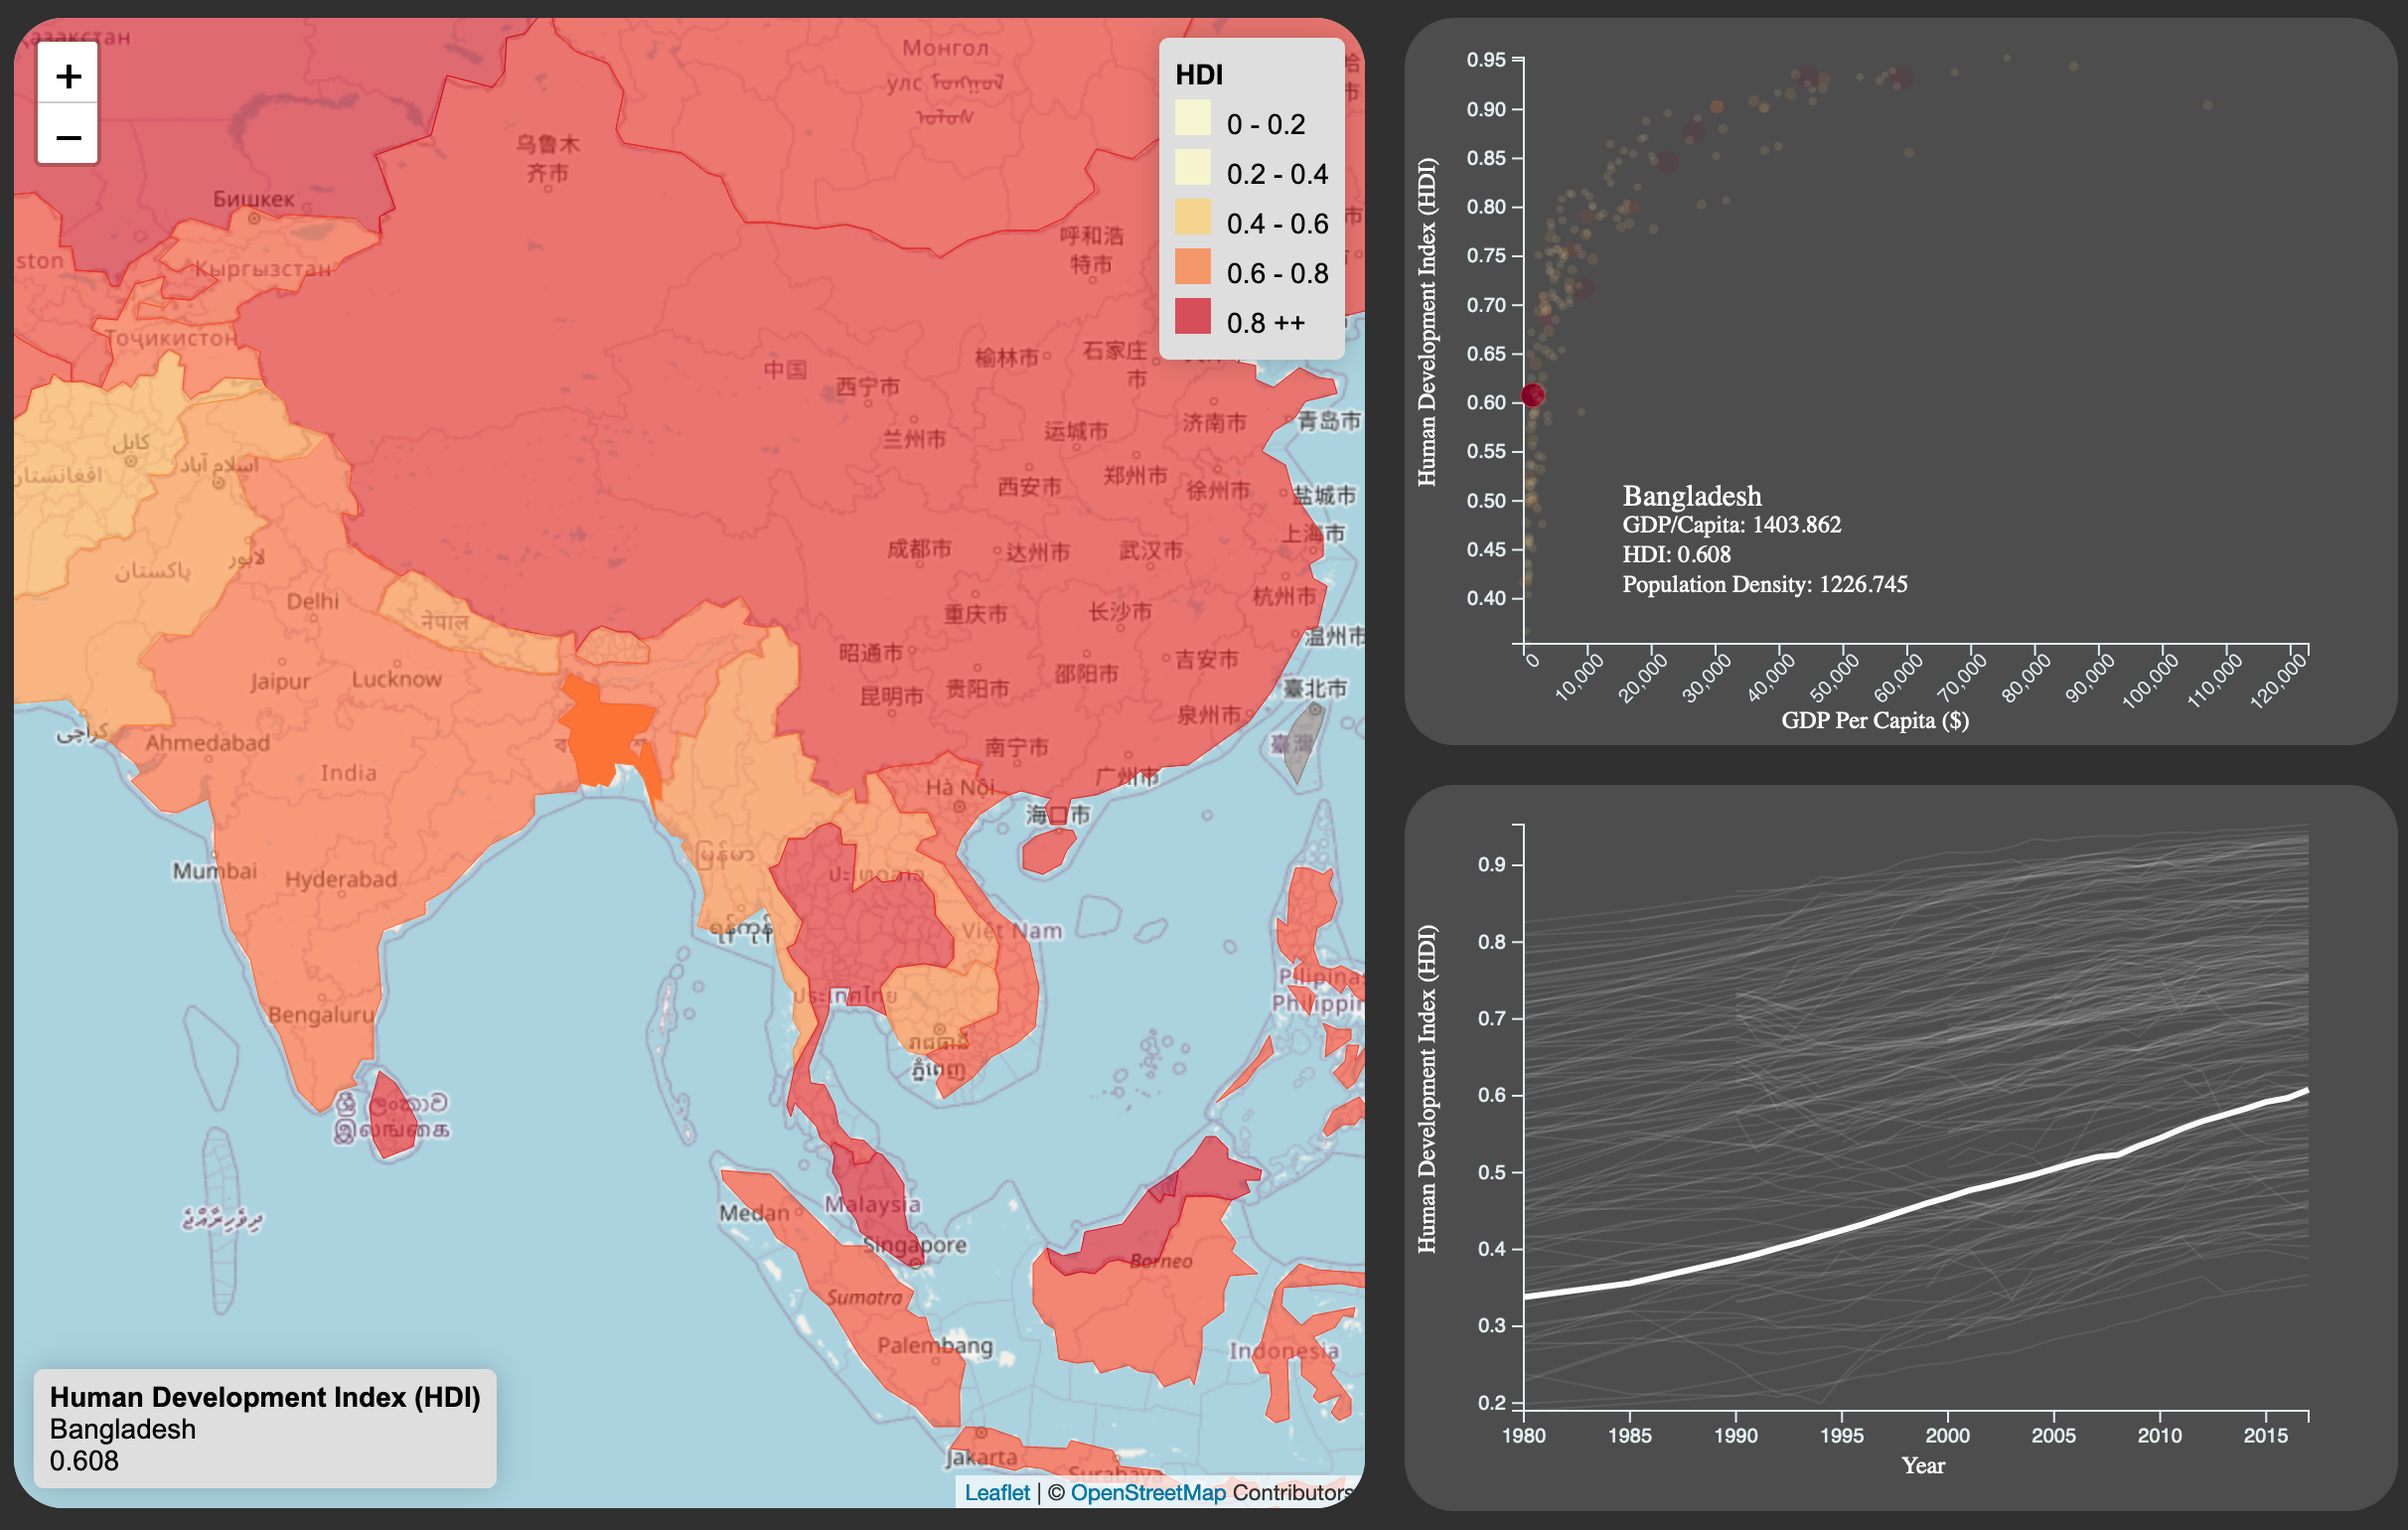
\includegraphics[height = 0.3\textwidth]{images/map_mouse_1.png}
    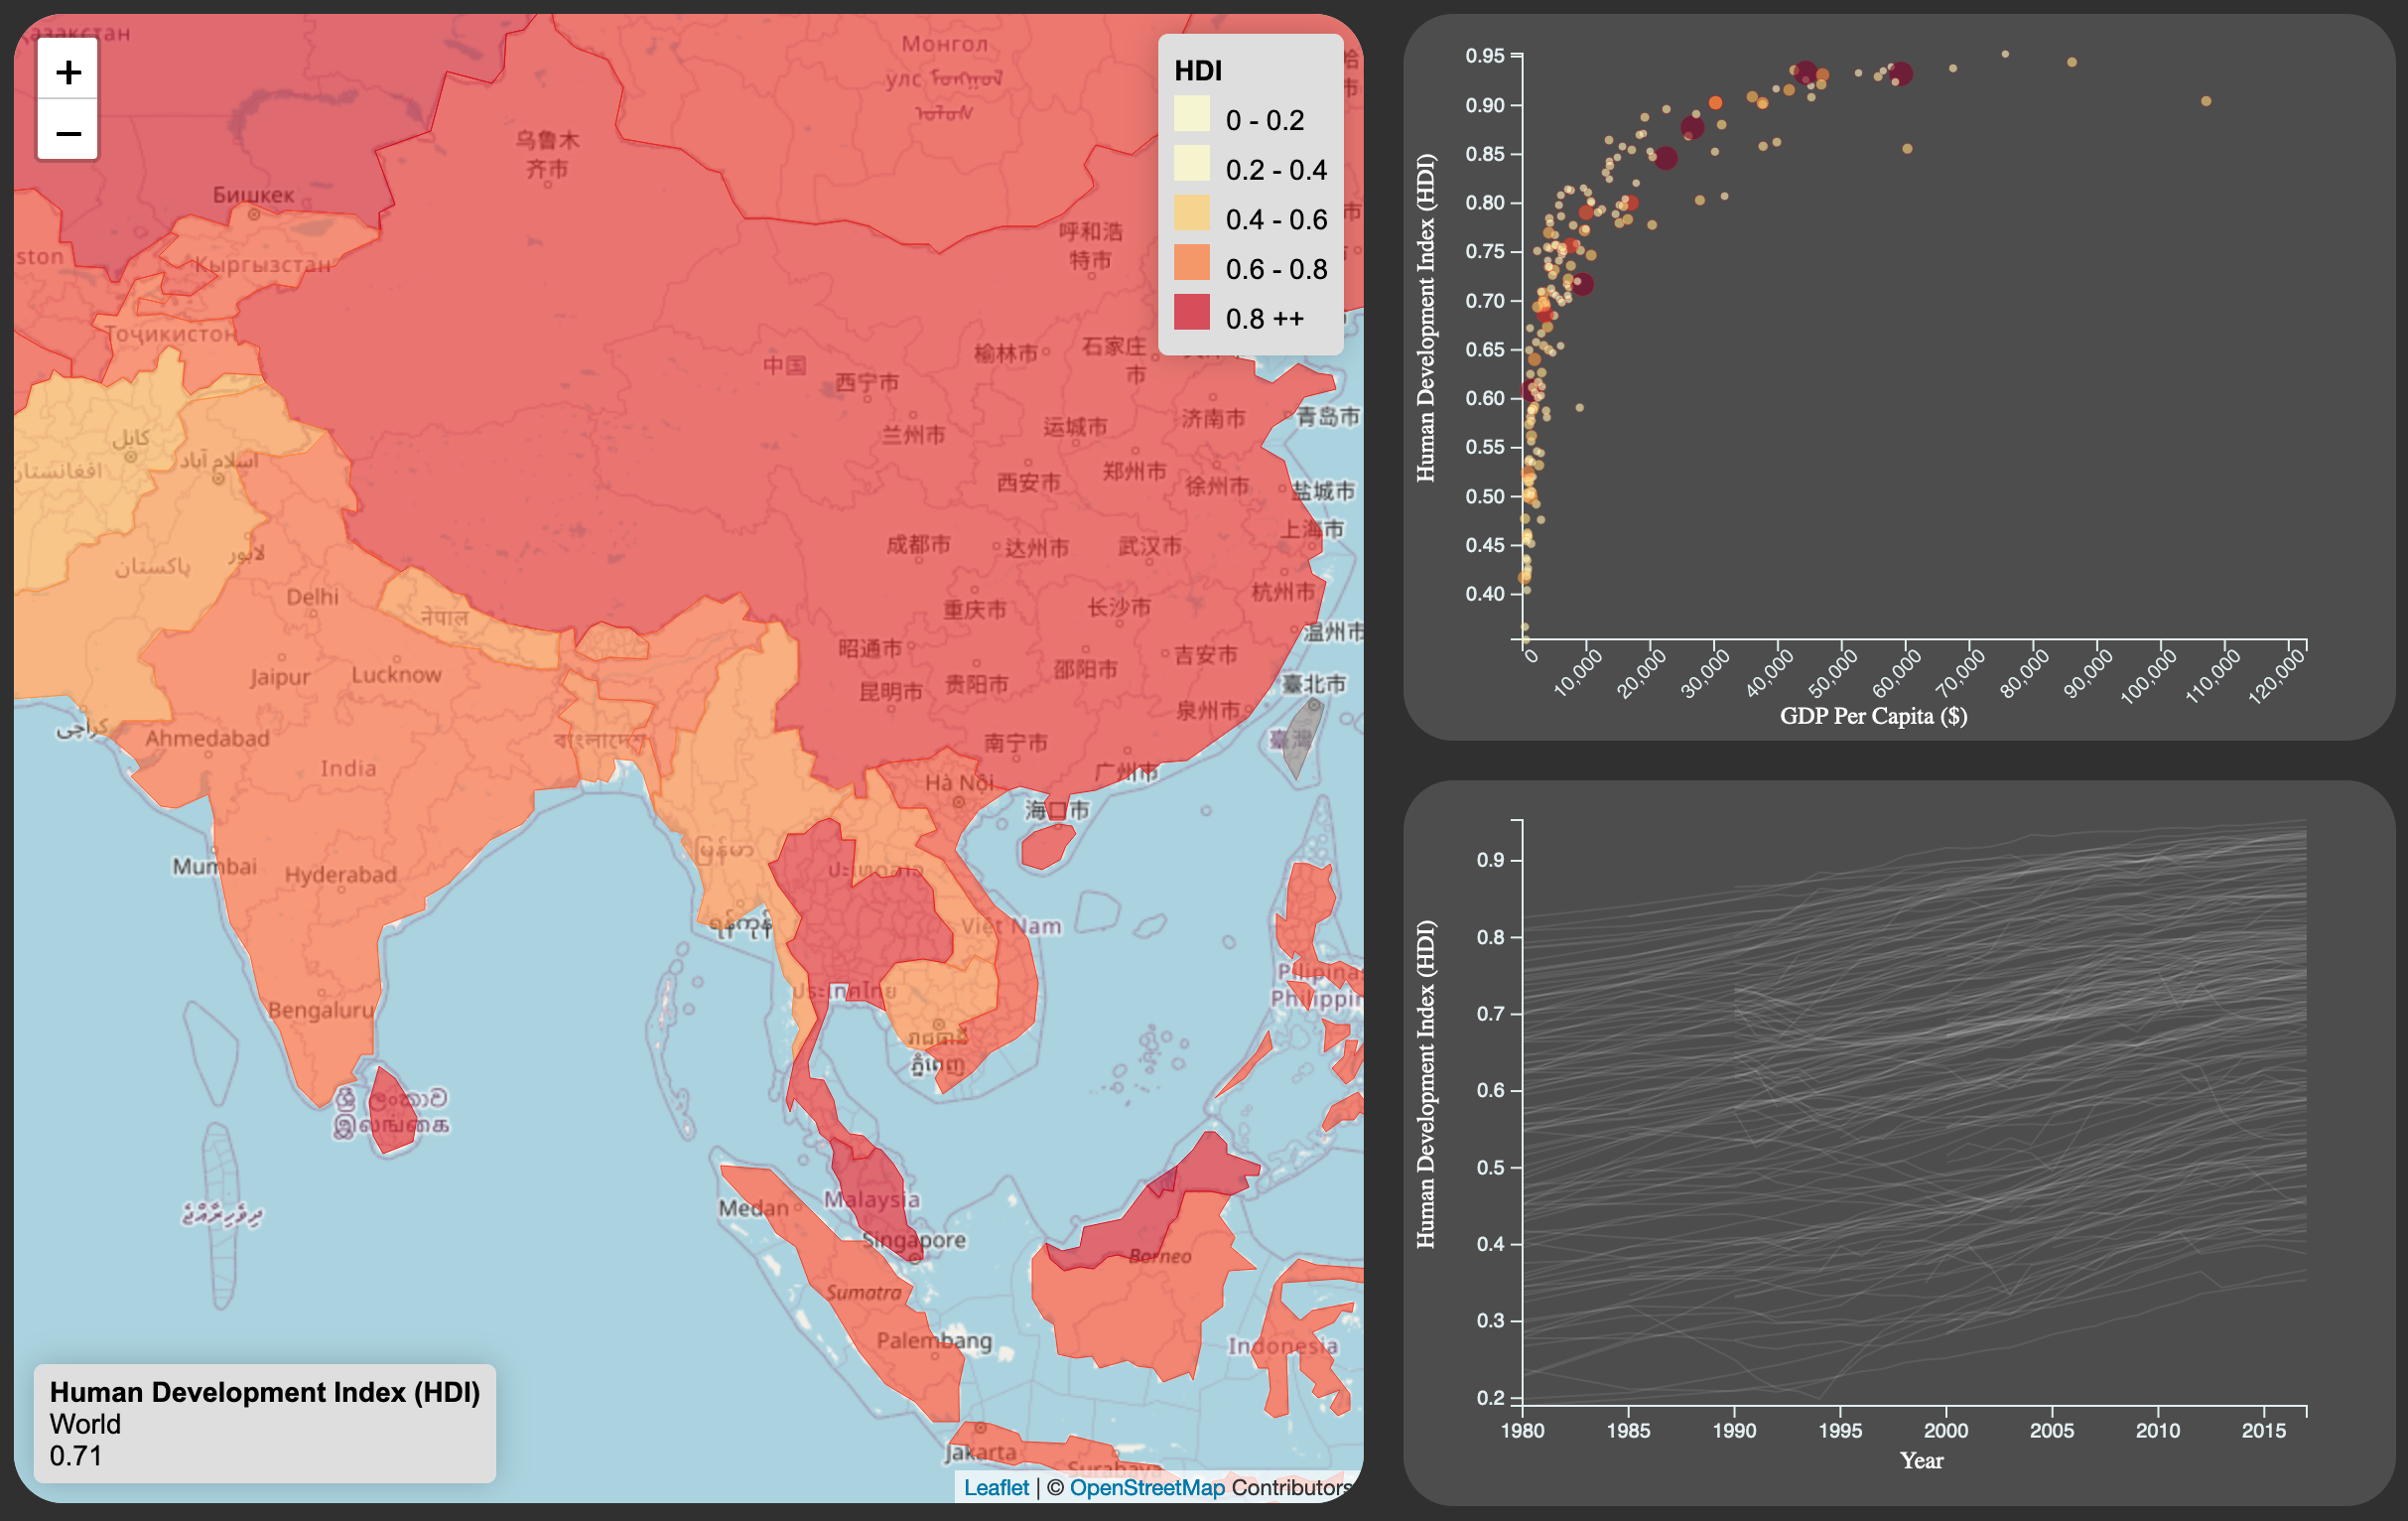
\includegraphics[height = 0.3\textwidth]{images/map_mouse_2.png}
    \label{fig:map-mouse-update}
    \caption{Map Mouse Update MouseOver and MouseOut}
\end{figure}
From figure \ref{fig:map-mouse-update}, we could see the parts of graph being updated as a result of the \verb|mouseOn| and \verb|mouseOut| events. Due to the nature of the computer's OS, the physical mouse is not visible during a screenshot, but the mouse is actually on the Bangladesh polygon on the map. 

Upon mouse over, the dynamic dashboard updates the following things:
\begin{itemize}
    \item Map: Highlight the selected country.
    \item Scatter Plot: Highlight the selected country, blur the rest of the countries, and show a detailed tooltip of the country's data, including the population density. 
    \item Line Chart: Highlight the selected country.
\end{itemize}

This is the same for all three visualizations on the dashboard. If the scatter plot is being interacted with, it would highlight the corresponding country on the map and update the line graph to show the country's change in HDI. The same would go for the line chart. 

\subsection{Map Zoom and Borders}
\begin{figure}[H]
    \centering
    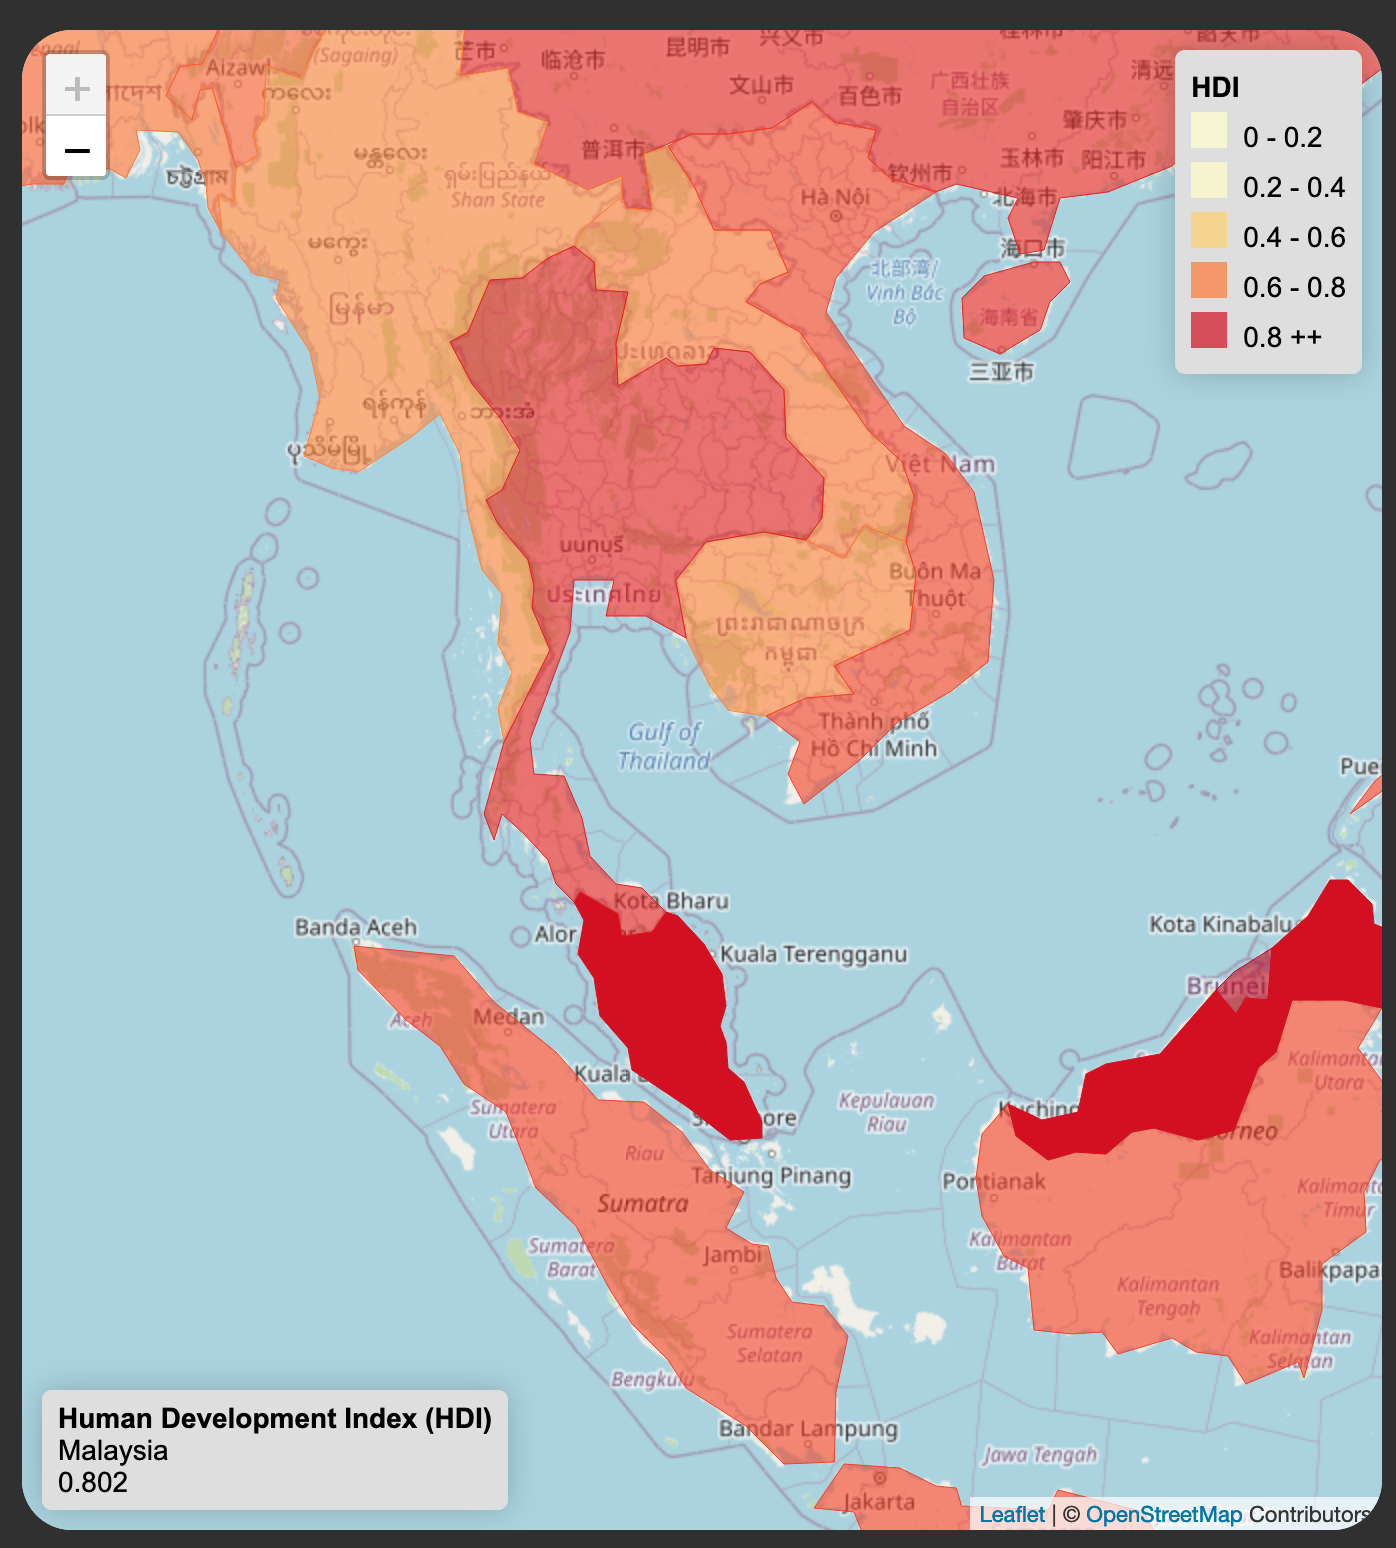
\includegraphics[height = 0.3\textwidth]{images/map_zoom_1.png}
    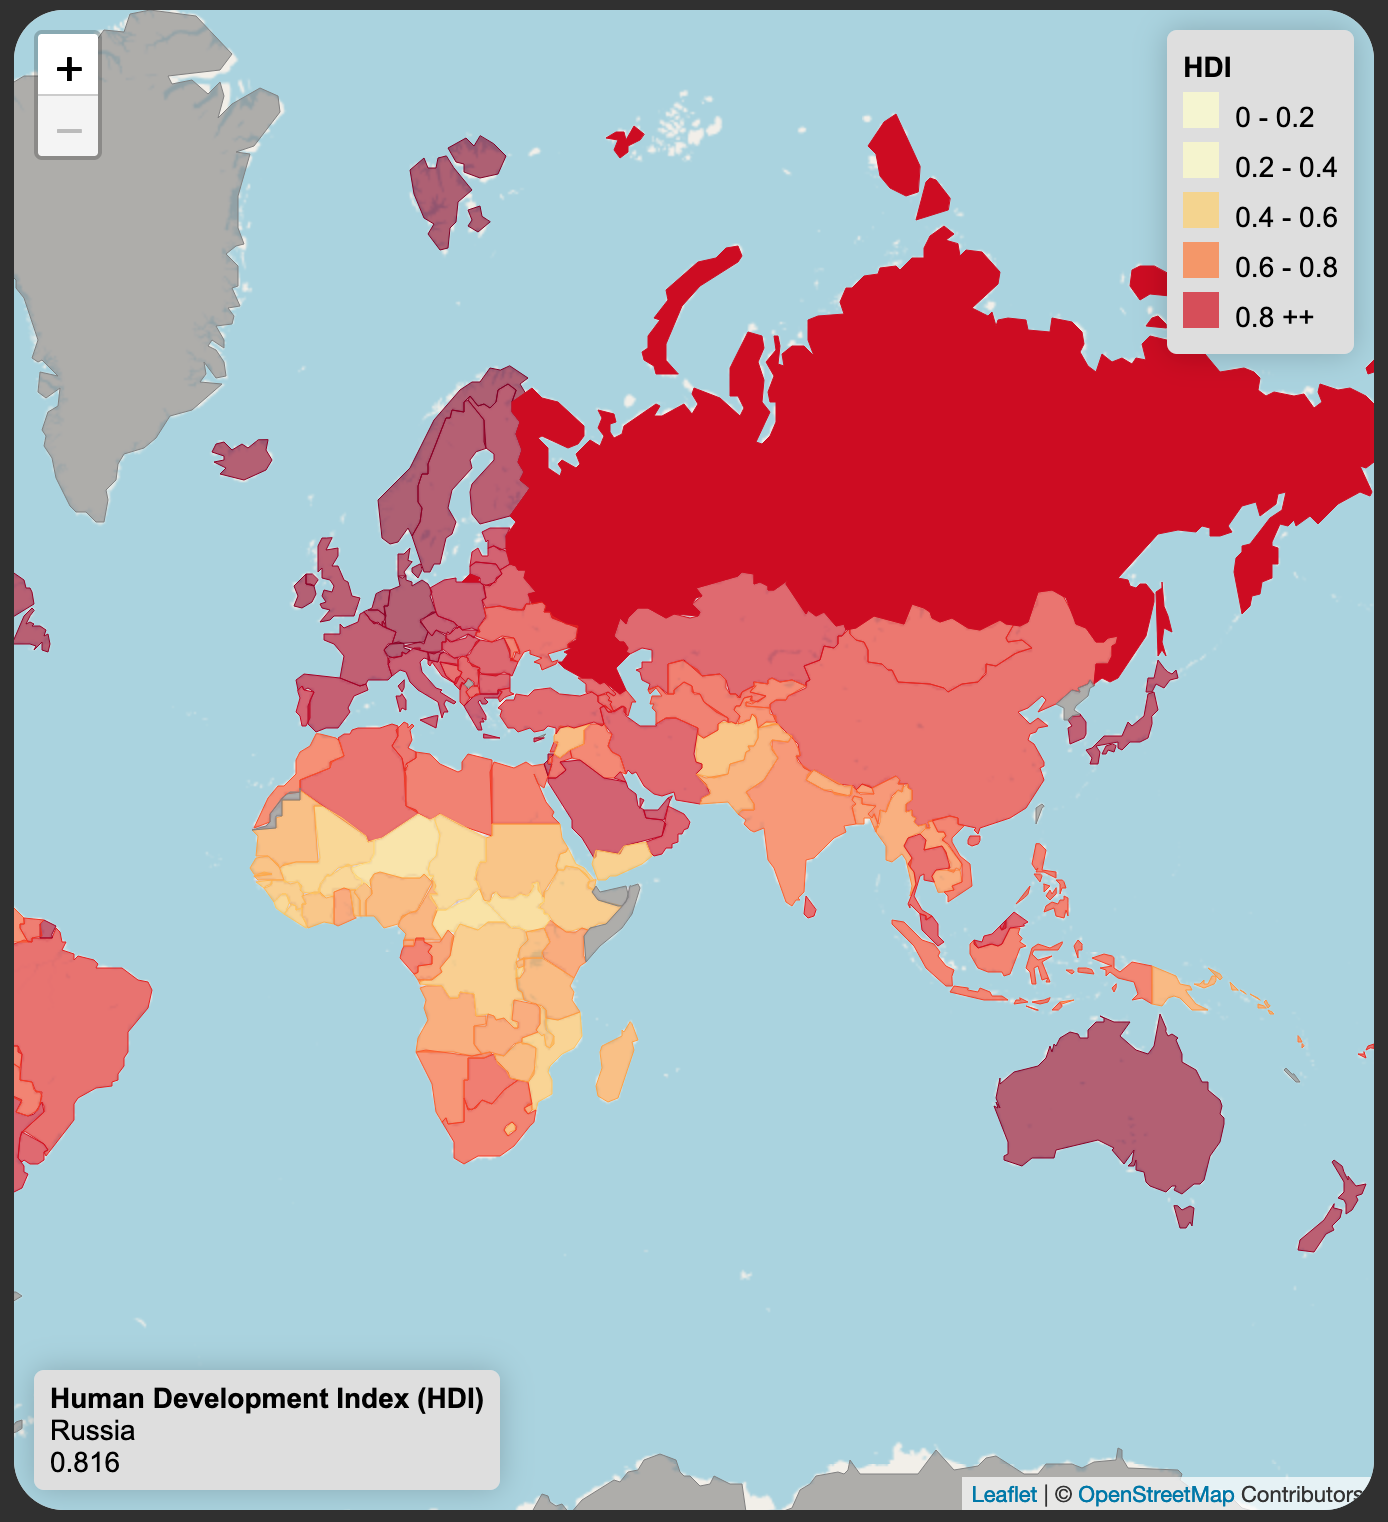
\includegraphics[height = 0.3\textwidth]{images/map_zoom_2.png}
    \label{fig:map-zoom}
    \caption{Map Minimum and Maximum Zoom}
\end{figure}
A border is being set for the map where if the user drags past the border, it would automatically bounce back. This is very hard to be shown, but the event could be tested out on the GitHub Page. From figure \ref{fig:map-zoom}, the user could see the minimum zoom level for the map just so that user could visualize changes to multiple countries. A maximum zoom was also set since the \verb|GeoJson| file used was one of a smaller scale to improve dashboard loading performance, hence, not being able to show in detail a country's detail. The zoom controls also greyed-out once a maximum zoom is reached. 

\section{Scatter Plot}
\begin{figure}[H]
    \centering
    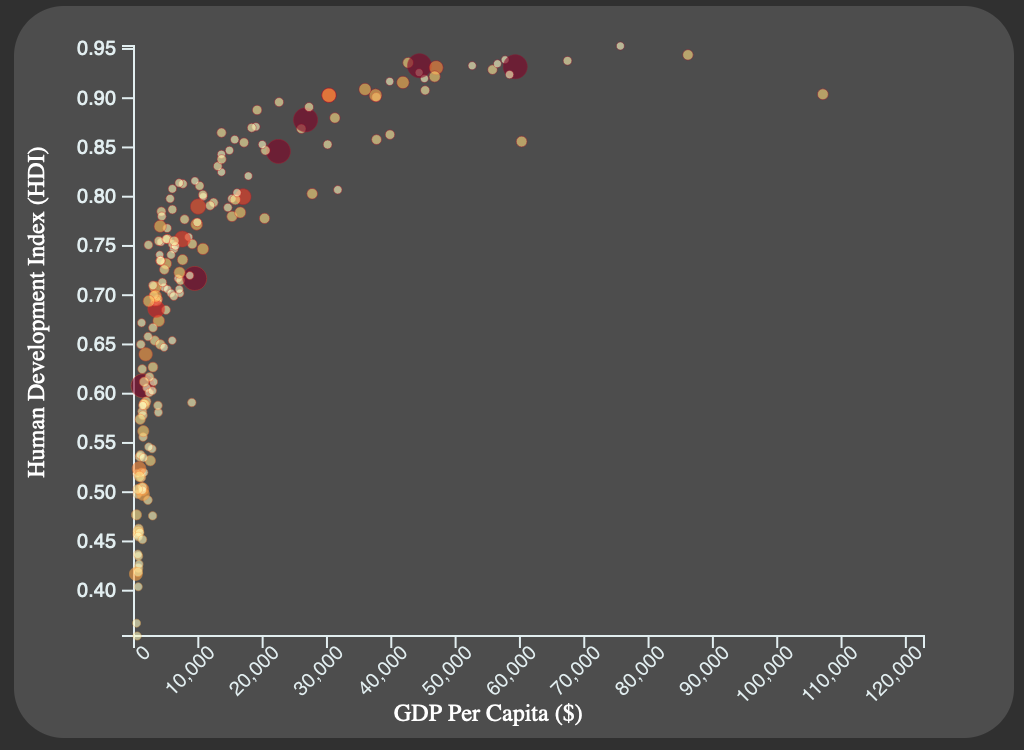
\includegraphics[height = 0.35\textwidth]{images/scatter_1.png}
    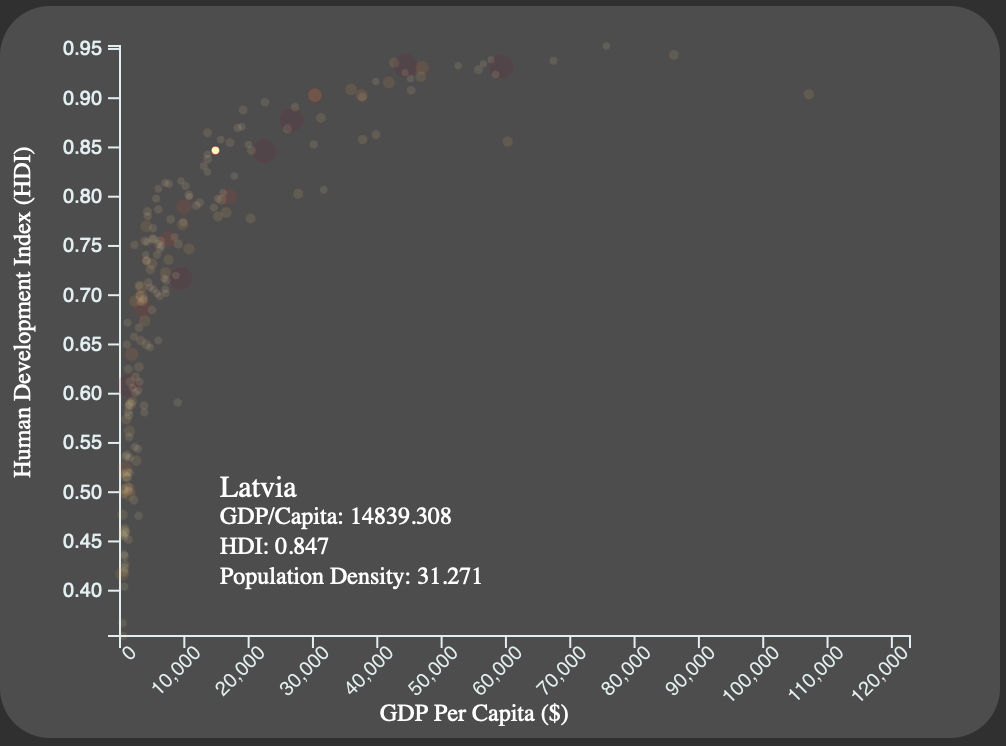
\includegraphics[height = 0.35\textwidth]{images/scatter_2.png}
    \label{fig:scatter}
    \caption{Map Minimum and Maximum Zoom}
\end{figure}
Figure \ref{fig:scatter} shows the scatter plot and what happens when the user hovers on a circle. The scatter plot was made solely using the \verb|d3.js| library. This was done using a \verb|enter()|-\verb|append()|-\verb|merge()|-\verb|exit()| function. This ensures that upon updating the year, the plots will transition its position. 
\begin{lstlisting}[label = {lst:scatter}, caption = {Scatter Plot Update}]
const u = scatterSvg.selectAll('circle')
                    .data(yearHdi);
...
// enter-append function
u.enter()
    .append('circle')
        .on('mouseover', mouseOver)
...
.merge(u)
    .transition()
        .duration(400)
            .attr('r', d => {
...
// remove extra stuff
u.exit()
    .transition()
            .duration(400)
            .remove();
\end{lstlisting}
The plot also shows three different types of data. The x-axis shows the GDP per Capita of the country, the y-axis shows the HDI, and the size of the circles are scaled to show the population density of a country. Once again, a unique id value has been assigned to each circle, to enable an effective way to update its style dynamically. 

From the scatter plot, we can conclude that HDI is indeed a viable development index as it shows a logarithmic correlation with the GDP/Capita indicator. This also shows that population density plays no role in determining how developed a country is. For instance, Hong Kong and Singapore are one of the most dense country in the world, yet they are two of the best performing countries in terms of HDI and GDP/Capital value. GDP/Capita also fails to capture the development levels of a country, as explained within the dashboard itself. 

\section{Line Chart}
From figure \ref{fig:map-mouse-update}, we could see the sole purpose of the line chart. is to show growth, using HDI values, for each individual country. There is an average upward trend for all countries, and this is just what we need to see in all parts of the world, where the countries should all be moving forwards, not back. 
\begin{lstlisting}[label = {lst:line}, caption = {Line Set Up}]
// add lines
for (let item of await getListOfCountry()) {
    ...
    // add the path
    linePlotSvg.append('path')
        .attr('class', 'hdi-line')
        .attr('id', `hdi-line-${item}`)
    ...
\end{lstlisting}

The way the lines were plotted was also slightly different. As shown in listing \ref{lst:line}, I have used a for loop for plot a line for each country there is, using the country code as a unique identifier to ease the update process. 

\section{Slider}
\begin{figure}[H]
    \centering
    
\includegraphics[width = 0.8\textwidth]{images/slider.png}
    \label{fig:slider}
    \caption{Slider}
\end{figure}
From figure \ref{fig:slider}, we could see a figure of the slider where it allows the user to slider along the slider to update the map and scatter plot the show data for the relevant years.
\begin{figure}[H]
    \centering
    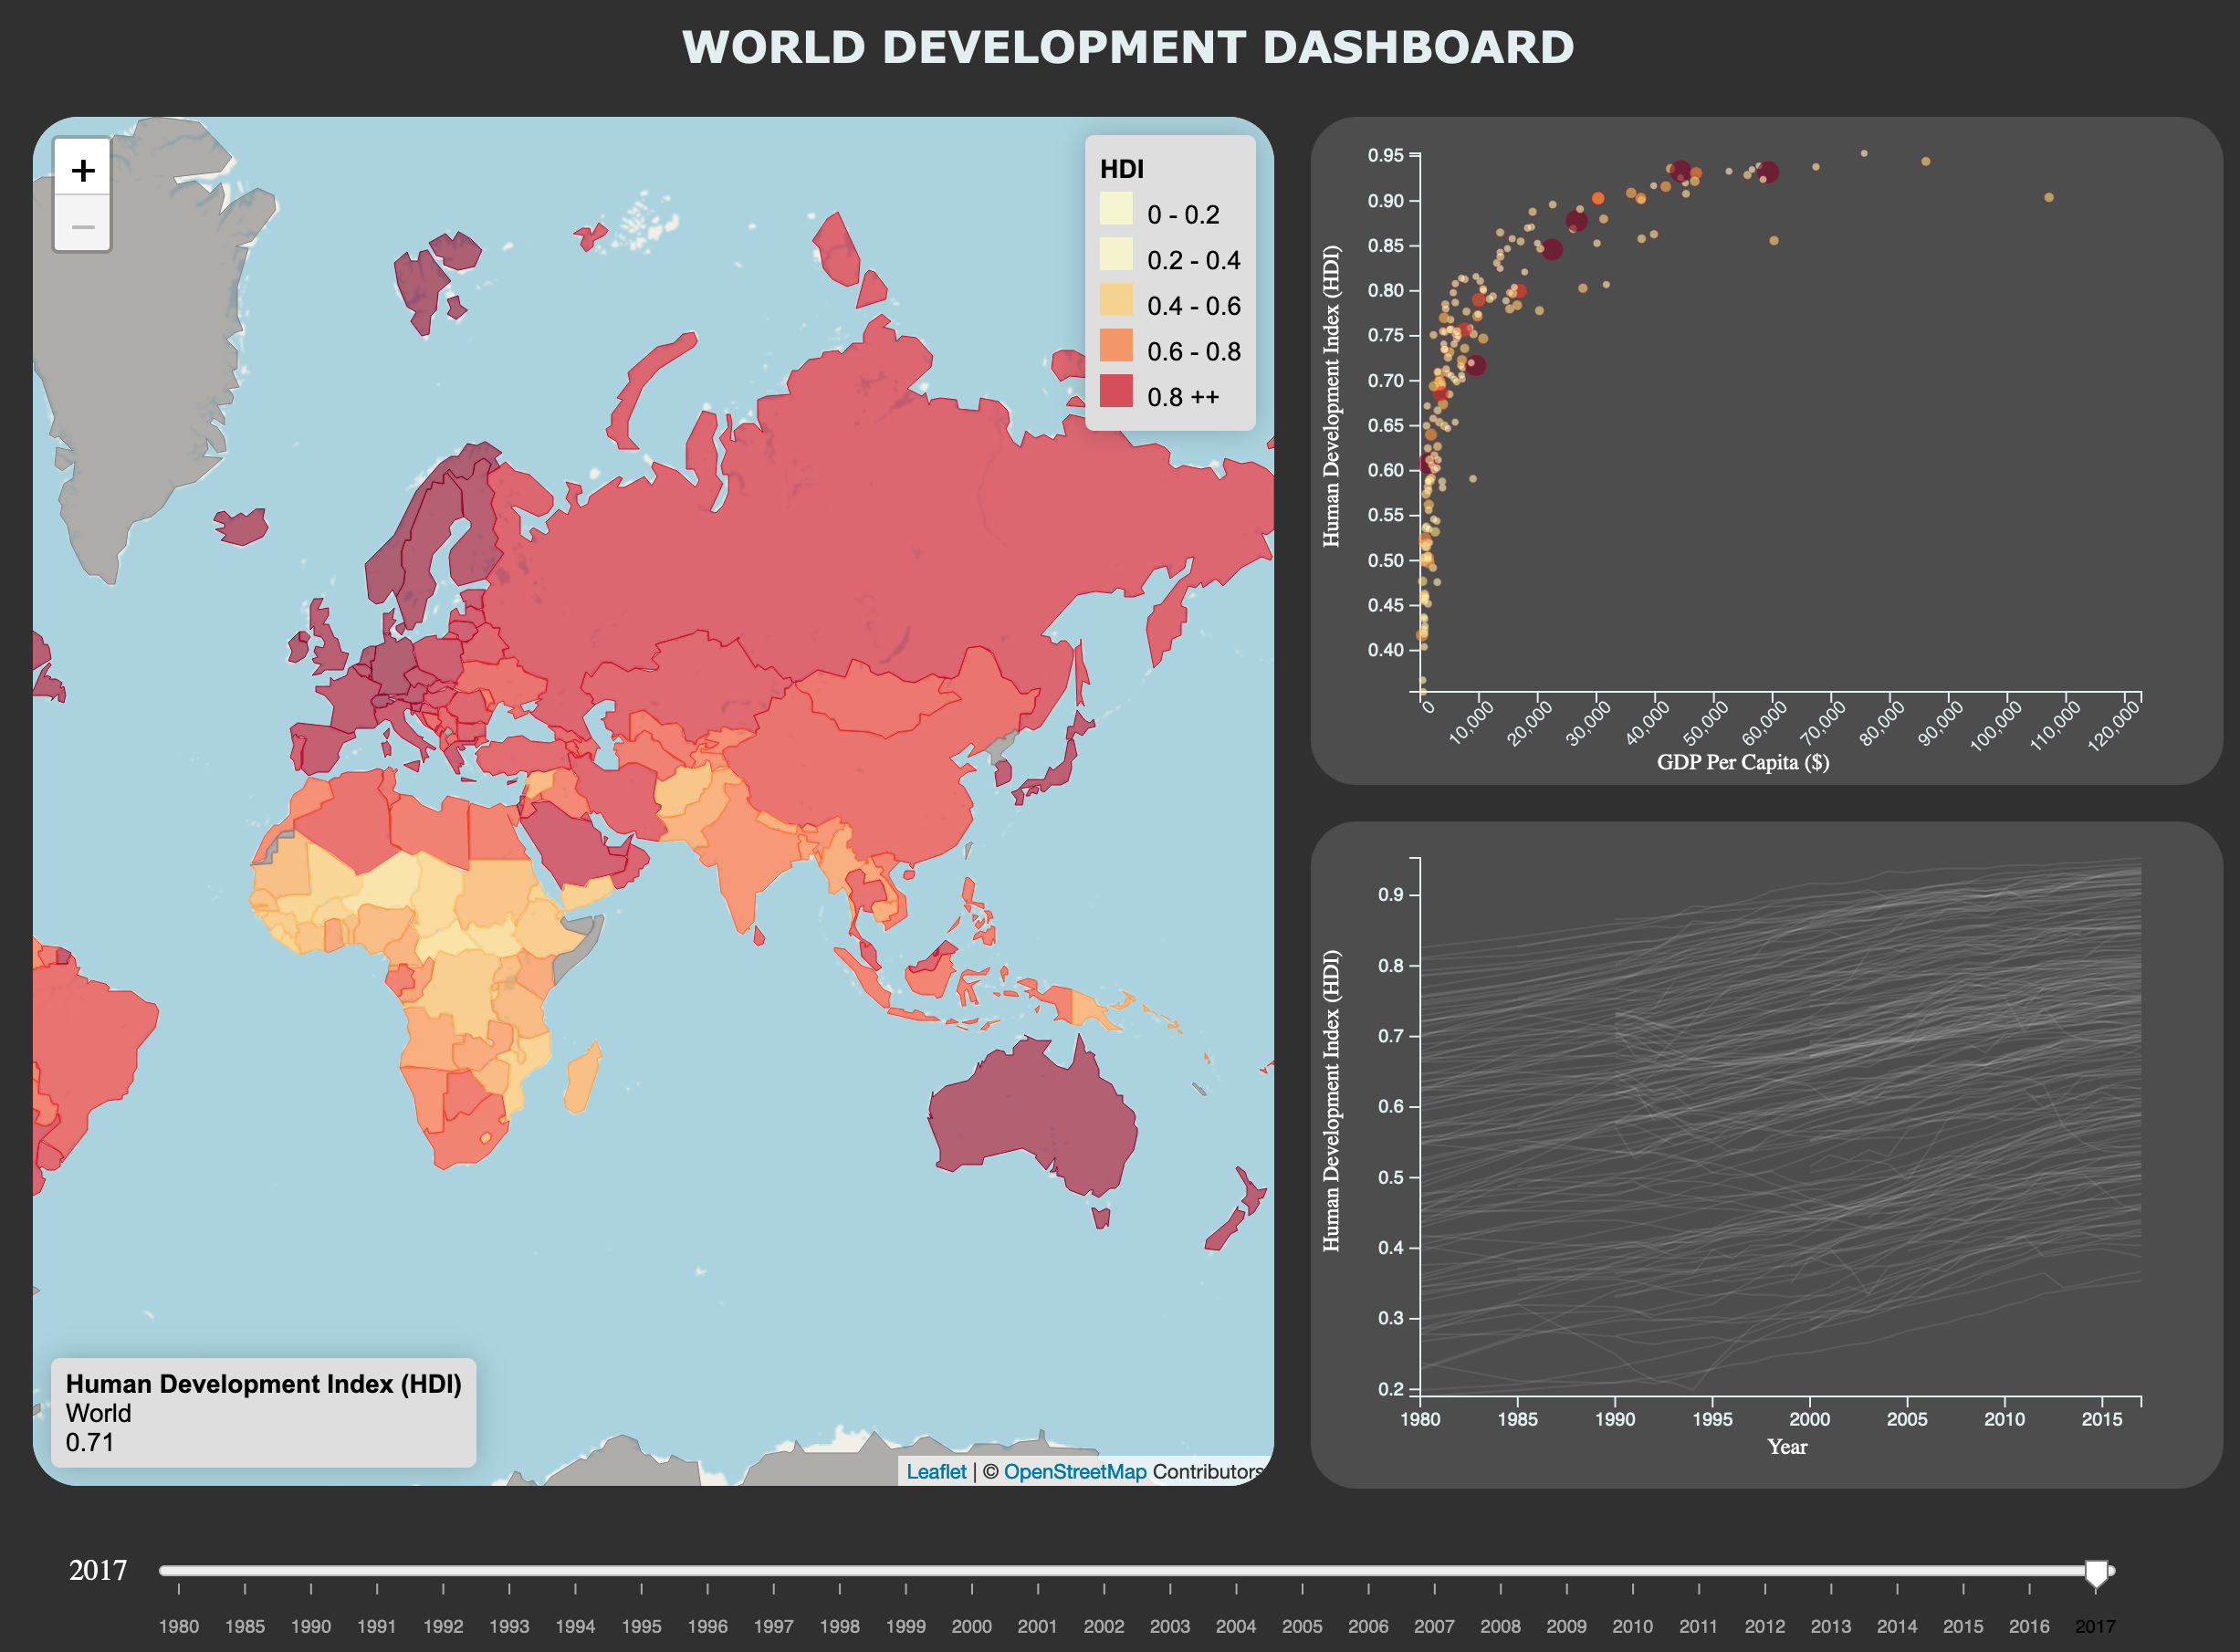
\includegraphics[width = 0.8\textwidth]{images/slider_2.png}
    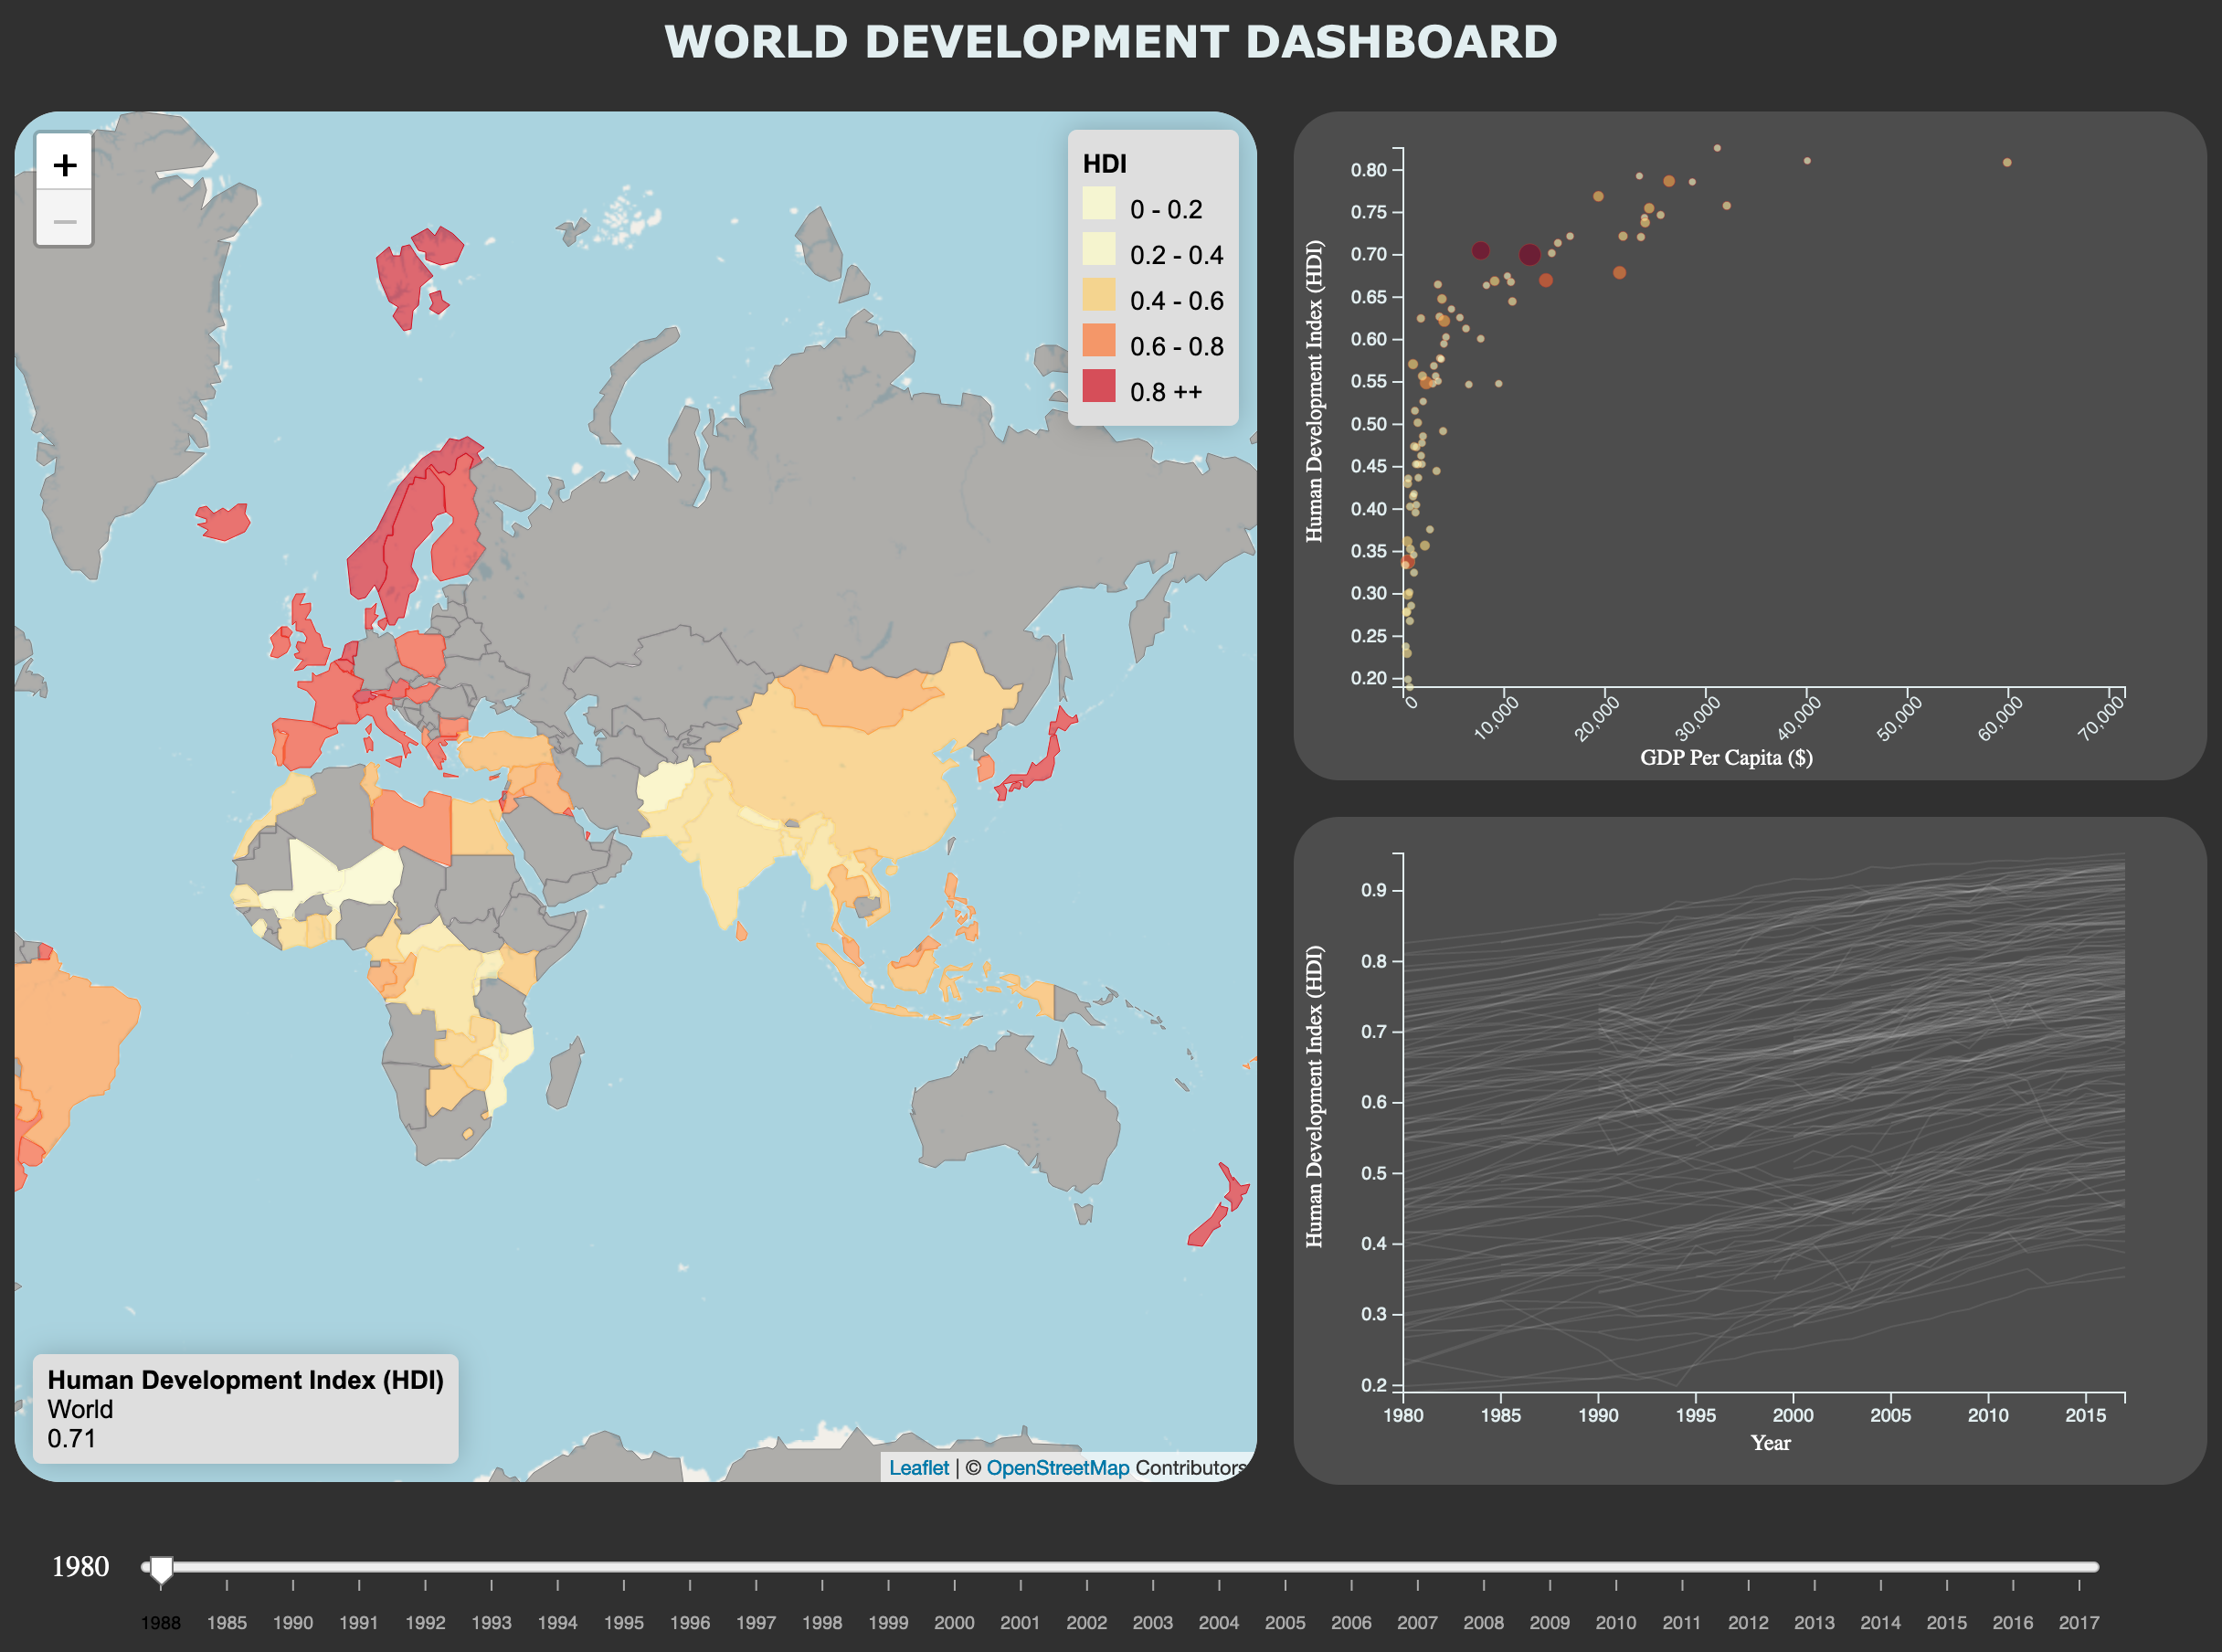
\includegraphics[width = 0.8\textwidth]{images/slider_1.png}
    \label{fig:slider-update}
    \caption{Slider update}
\end{figure}
Figure \ref{fig:slider-update} shows what happens the  map and scatter plot upon update of the slider. The default slider position is as 2017, and upon sliding the controls to 1980, the map and scatter plot immediately shows a few extra countries without HDI data. This is due to the fact that HDI was not really a thing up till the early 2000s, as shown in the line chart|multiple countries have lines only starting at 2000. \\
\lstinputlisting[firstline = 46, lastline = 57, label = {lst:dash0-pdate}, caption = {Update function for the dash}]{../../public/js/part4/functions.js}
The update is done by an \verb|updateDashboard()| function, as shown in listing \ref{lst:dash0-pdate}. Upon change of the slider, the changed value (new year value) is being passed on to the \verb|updateDashboard()| function, where it updates a global \verb|window.year| variable, and it is just a remaining task of simply calling the \verb|update()| function for each of the map and scatter module. 

\section{Contents and Footer Section}
\begin{figure}[H]
    \centering
    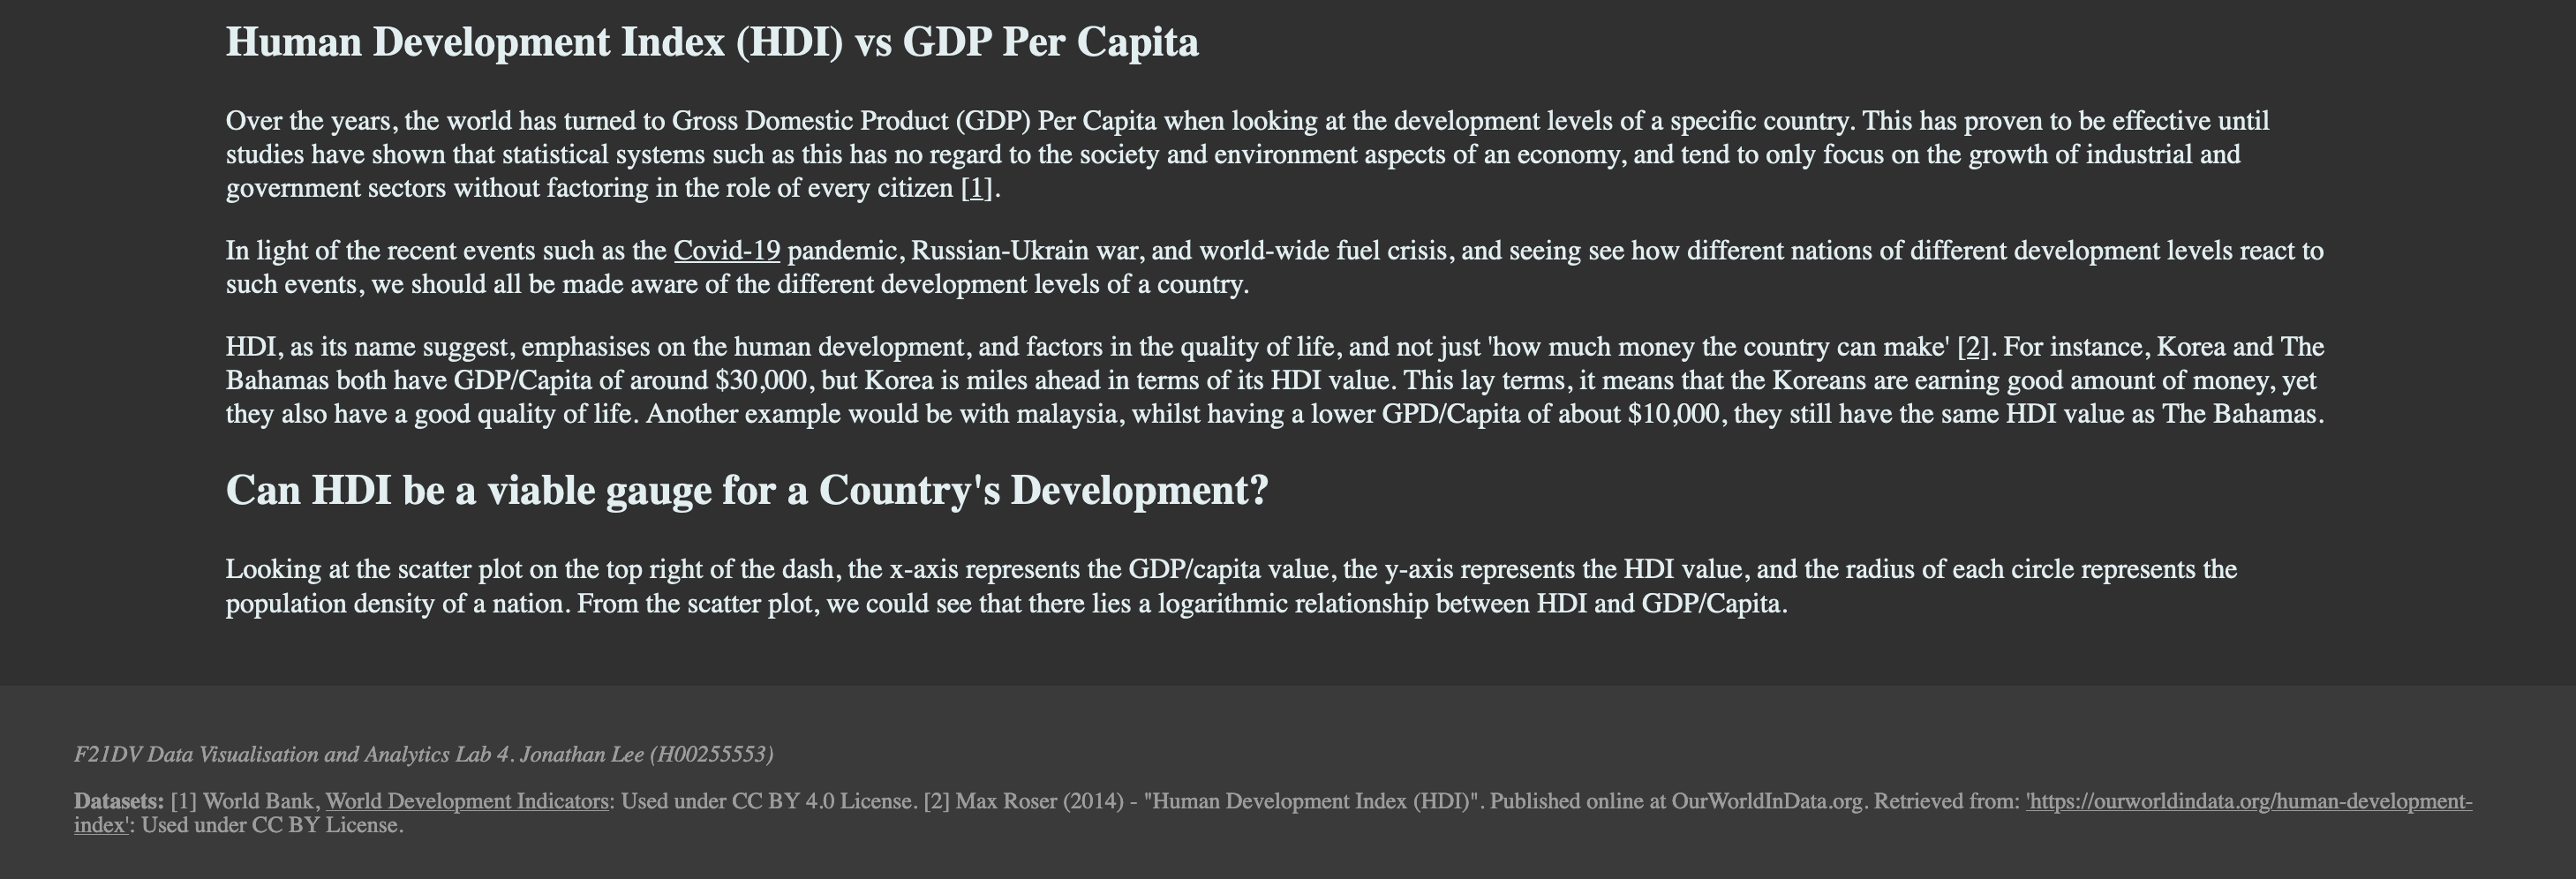
\includegraphics[width = 0.8\textwidth]{images/content.png}
    \label{fig:content}
    \caption{Content and Footer}
\end{figure}
The content and footer section is simply just a basic html knowledge, where its purpose is to provide valuable explanation for the dashboard. I have created a generic function that can be used to add divs systematically into the container. This is as shown as below, both the function, and its implementation.
\lstinputlisting[firstline = 6, lastline = 51, label = {lst:content}, caption = {Content Section}]{../../public/js/part4/content.js}

\chapter{Conclusion}
In conclusion, through the 4 Labs, I have now a more robust understanding of Visualizations and particularly through the most intuitive and accessible manner|through a web application. My understanding of \verb|d3.js|, best programming practices, and DOM has been deepened as well.

\end{document}